%%%%%%%%%%%%%%%%%%%%%%%%%%%%%%%%%%%%%%%%%%%%%%%%%%%%%%%%%%%%%%%%%%%%%%%%%%%%%%%
% PREAMBOLO COMUNE PER APPUNTI (Stile Scuro)
%
% Questo file contiene tutte le impostazioni e i pacchetti comuni.
% NON contiene \begin{document} o \end{document}.
%
% Istruzioni per la compilazione del file principale:
% pdflatex -shell-escape nomefile_principale.tex
%%%%%%%%%%%%%%%%%%%%%%%%%%%%%%%%%%%%%%%%%%%%%%%%%%%%%%%%%%%%%%%%%%%%%%%%%%%%%%%

\documentclass{article}

% --- Encoding e lingua ---
\usepackage[utf8]{inputenc}
\usepackage[italian]{babel}

% --- Margini e layout ---
\usepackage{geometry}
\geometry{a4paper, margin=1in}

% --- Font sans-serif (come Helvetica) ---
\usepackage[scaled]{helvet}
\renewcommand{\familydefault}{\sfdefault}
\usepackage[T1]{fontenc}

% --- Matematica ---
\usepackage{amsmath}
\usepackage{amssymb}

% --- Liste personalizzate ---
\usepackage{enumitem}
% \setlist{nosep}

% --- Immagini e Grafica ---
\usepackage{float}
% \usepackage{graphicx}
\usepackage{tikz}
\usetikzlibrary{shapes.geometric, positioning, arrows.meta, calc, fit, backgrounds, patterns, decorations.pathreplacing}

% --- Tabelle Avanzate ---
\usepackage{array}
\usepackage{booktabs}
\usepackage{longtable}

% --- Hyperlink e Metadati PDF ---
\usepackage{hyperref}

\hypersetup{
    colorlinks=true,
    linkcolor=white,
    filecolor=magenta,
    urlcolor=cyan,
    citecolor=green,
    % pdftitle, pdfauthor, ecc. verranno impostati nel file principale
    pdfpagemode=FullScreen,
    bookmarksopen=true,
    bookmarksnumbered=true
}

% --- Licenza del documento ---
\usepackage[
  type={CC},
  modifier={by-sa},
  version={4.0},
]{doclicense}

% --- Colori e Sfondo Nero ---
\usepackage{xcolor}
\pagecolor{black}
\color{white}

% --- Evidenziazione del Codice ---
\usepackage{minted}
\setminted{
    frame=lines,
    framesep=2mm,
    fontsize=\small,
    breaklines=true,
    style=monokai,
    bgcolor=black!80
}
\usemintedstyle{monokai}

% --- Comandi personalizzati per algebra relazionale ---
\newcommand{\Rel}[1]{\textit{#1}} % Per i nomi delle relazioni
\newcommand{\Attr}[1]{\textsf{#1}} % Per i nomi degli attributi

\newcommand{\myunion}{\cup}
\newcommand{\myintersection}{\cap}
\newcommand{\mydifference}{-}
\newcommand{\myrename}[2]{\rho_{#1}(#2)}
\newcommand{\myselectop}[2]{\sigma_{#1}(#2)}
\newcommand{\myproject}[2]{\pi_{#1}(#2)}
\newcommand{\mycartesian}{\times}
\newcommand{\mynaturaljoin}{\bowtie} % Usare \Join da amssymb se disponibile e preferito
\newcommand{\mythetajoin}[3]{#1 \bowtie_{#2} #3} % R1 \bowtie_cond R2

% --- Comandi personalizzati per logica ---
\newcommand{\mylandop}{\wedge}
\newcommand{\myvel}{\vee}
\newcommand{\mynegop}{\neg}
\newcommand{\myforallop}{\forall}
\newcommand{\myexistsop}{\exists}

% --- Join esterni (outer join) ---
% Definizione standard per i join esterni
\def\ojoin{\setbox0=\hbox{$\mynaturaljoin$}%
	\rule[-.02ex]{.25em}{.4pt}\llap{\rule[\ht0]{.25em}{.4pt}}}
\newcommand{\myleftouterjoin}{\mathbin{\ojoin\mkern-5.8mu\mynaturaljoin}}
\newcommand{\myrightouterjoin}{\mathbin{\mynaturaljoin\mkern-5.8mu\ojoin}}
\newcommand{\myfullouterjoin}{\mathbin{\ojoin\mkern-5.8mu\mynaturaljoin\mkern-5.8mu\ojoin}}



% --- Titolo ---
\title{Guida alla Risoluzione degli Esercizi di Reti di Calcolatori}
\author{Basato sulle slide del Prof. Luciano Bononi}
\date{\today}

\begin{document}

\maketitle
\tableofcontents
\newpage


\section*{Indice delle Tipologie di Esercizi:}
\begin{enumerate}[label=\arabic*.] % Lista numerata con margine allineato
    \item \hyperref[sec:ipv4-subnetting]{Indirizzamento IPv4 e Subnetting (VLSM)}
    \item \hyperref[sec:protocolli-sicuri]{Progettazione di Protocolli di Comunicazione Sicura (Alice \& Bob)}
    \item \hyperref[sec:wireless]{Comunicazioni Wireless (Link Budget, OFDM, Fresnel)}
    \item \hyperref[sec:openflow]{Configurazione Tabelle OpenFlow}
    \item Analisi e Interpretazione di Output/Configurazioni di Rete (DNS, PING, URL) % Placeholder, sezione da aggiungere
    \item Calcolo Prestazioni di Rete (Throughput, Latenza, Congestione) % Placeholder, sezione da aggiungere
    \item Routing (Algoritmo di Dijkstra) % Placeholder, sezione da aggiungere
    \item Codifica del Segnale Wireless % Placeholder, sezione da aggiungere
\end{enumerate}

\hrule % Linea orizzontale come separatore

% --- Sezione 1: Indirizzamento IPv4 e Subnetting (VLSM) ---
\section{Indirizzamento IPv4 e Subnetting (VLSM)} % Sezione principale
\label{sec:ipv4-subnetting} % Etichetta per riferimenti incrociati

\subsection{Concetti Chiave}
\begin{itemize} % Lista puntata con margine allineato
    \item \textbf{Indirizzo IP:} Identificatore univoco di un host in una rete.
    \item \textbf{Netmask (Maschera di Sottorete):} Divide l'indirizzo IP in parte di rete e parte di host.
    \item \textbf{CIDR (Classless Inter-Domain Routing):} Notazione \texttt{/n} che indica i primi \texttt{n} bit come parte di rete.
    \item \textbf{Indirizzo di Rete:} Primo indirizzo di un range, con tutti i bit della parte host a 0. Non assegnabile a host.
    \item \textbf{Indirizzo di Broadcast:} Ultimo indirizzo di un range, con tutti i bit della parte host a 1. Invia dati a tutti gli host della sottorete. Non assegnabile a host.
    \item \textbf{Indirizzi Host Validi:} Indirizzi compresi tra l'indirizzo di rete e quello di broadcast. Numero di host = $2^{(32-n)} - 2$.
    \item \textbf{VLSM:} Tecnica che permette di usare maschere di sottorete di lunghezza variabile per ottimizzare l'uso degli indirizzi IP, creando sottoreti di dimensioni diverse in base alle necessità.
\end{itemize}

\subsection{Procedura di Svolgimento (VLSM - Esercizio 9 tipico)}
\begin{enumerate}[label=\arabic*.]
    \item \textbf{Analisi Requisiti:} Identifica il numero massimo di host richiesto per ogni sottorete.
    \item \textbf{Ordinamento:} Ordina le sottoreti in base al numero di host richiesti, dalla più grande alla più piccola. Questo aiuta a prevenire la frammentazione dello spazio di indirizzamento.
    \item \textbf{Calcolo Bit Host:} Per ogni sottorete, calcola il numero minimo di bit $h$ necessari per la parte host: $2^h - 2 \ge \text{numero\_host\_richiesti}$. La maschera sarà $32 - h$.
    \item \textbf{Allocazione Spazio:} Partendo dall'indirizzo di rete generale fornito (o da un blocco scelto):
    \begin{itemize}
        \item Alloca il primo blocco contiguo di indirizzi sufficiente per la sottorete più grande.
        \item Calcola: Indirizzo di Rete, Primo Host, Ultimo Host, Indirizzo di Broadcast, IP del Router (solitamente il primo o l'ultimo host valido della sottorete, o uno specifico se indicato).
        \item L'indirizzo successivo al broadcast della sottorete appena creata diventa l'inizio del blocco disponibile per la successiva.
    \end{itemize}
    \item \textbf{Iterazione:} Ripeti il punto 4 per tutte le sottoreti, allocando blocchi contigui.
    \item \textbf{Router IP:} Assegna gli IP ai router. Un router che connette più sottoreti avrà un IP per ogni interfaccia su quella sottorete. L'IP del router è spesso il Default Gateway per gli host di quella sottorete.
    \item \textbf{Verifica:} Assicurati che i range di indirizzi delle sottoreti non si sovrappongano.
\end{enumerate}

\subsection{Formule Utili}
\begin{itemize}
    \item Numero host disponibili: $2^h - 2$ (dove $h$ sono i bit per la parte host)
    \item Netmask da $h$: $32 - h$ bit a 1.
    \item Indirizzo di Rete: $\text{IP AND Netmask}$
    \item Indirizzo di Broadcast: $\text{IndirizzoRete OR (NOT Netmask)}$ (o più semplicemente, l'indirizzo prima della rete successiva).
    \item Primo Host: $\text{IndirizzoRete} + 1$
    \item Ultimo Host: $\text{IndirizzoBroadcast} - 1$
\end{itemize}

\begin{table}[h]
\centering
\begin{tabular}{|c|c|c|c|c|c|}
\hline
\rowcolor{bg_custom}
\textbf{CIDR} & \textbf{Subnet Mask} & \textbf{Host Bits} & \textbf{Host Disp.} & \textbf{Classe} & \textbf{Range Pattern} \\
\hline
\rowcolor{bg_custom_2}
/8  & 255.0.0.0 & 24 & 16777214 & A & x.[0-255].[0-255].[0-255] \\
\hline
/16 & 255.255.0.0 & 16 & 65534 & B & x.x.[0-255].[0-255] \\
\hline
\rowcolor{bg_custom_2}
/17 & 255.255.128.0 & 15 & 32766 & & x.x.[0-127/128-255].[0-255] \\
\hline
/18 & 255.255.192.0 & 14 & 16382 & & x.x.[0,64,128,192].[0-255] \\
\hline
\rowcolor{bg_custom_2}
/19 & 255.255.224.0 & 13 & 8190 & & x.x.[0,32,64,...,224].[0-255] \\
\hline
/20 & 255.255.240.0 & 12 & 4094 & & x.x.[0,16,32,...,240].[0-255] \\
\hline
\rowcolor{bg_custom_2}
/21 & 255.255.248.0 & 11 & 2046 & & x.x.[0,8,16,...,248].[0-255] \\
\hline
/22 & 255.255.252.0 & 10 & 1022 & & x.x.[0,4,8,...,252].[0-255] \\
\hline
\rowcolor{bg_custom_2}
/23 & 255.255.254.0 & 9  & 510 & & x.x.y.[0-255] (y pari) \\
\hline
/24 & 255.255.255.0 & 8  & 254 & C & x.x.x.[0-255] \\
\hline
\rowcolor{bg_custom_2}
/25 & 255.255.255.128 & 7  & 126 & & x.x.x.[0-127/128-255] \\
\hline
/26 & 255.255.255.192 & 6  & 62 & & x.x.x.[0,64,128,192] \\
\hline
\rowcolor{bg_custom_2}
/27 & 255.255.255.224 & 5  & 30 & & x.x.x.[0,32,64,...,224] \\
\hline
/28 & 255.255.255.240 & 4  & 14 & & x.x.x.[0,16,32,...,240] \\
\hline
\rowcolor{bg_custom_2}
/29 & 255.255.255.248 & 3  & 6 & & x.x.x.[0,8,16,...,248] \\
\hline
/30 & 255.255.255.252 & 2  & 2 & & x.x.x.[0,4,8,...,252] \\
\hline
\end{tabular}
\caption{Mappatura CIDR a subnet mask e numero di host ($2^h - 2$ dove $h$ = bit host). La x indica qualsiasi valore valido (0-255).}
\end{table}

\subsection{Esempio Svolto (basato su Esercizio 9, "Scritto 26 Maggio 2023" e "Scritto Reti Di Calcolatori 2024-30-31")}
Prendiamo l'esercizio 9 della prova del 26 Maggio 2023.
\texttt{Network N = 177.34.146.0/23}
\begin{itemize}
    \item \textbf{Netmask N:} \texttt{/23} $\to$ \texttt{255.255.254.0} (11111111.11111111.11111110.00000000)
    \item \textbf{Rete N:} \texttt{177.34.146.0}
    \item \textbf{Bit host per N:} $32 - 23 = 9$ bit. Host totali: $2^9 = 512$. Host validi: $510$.
    \item \textbf{Range N:} \texttt{177.34.146.0} - \texttt{177.34.147.255}
    \item \textbf{Primo Host N:} \texttt{177.34.146.1}
    \item \textbf{Ultimo Host N (o Router IP N):} \texttt{177.34.147.254}
    \item \textbf{Broadcast N:} \texttt{177.34.147.255}
\end{itemize}

Ora suddividiamo. Supponiamo le richieste (come da figura ma invento i numeri per semplicità, tu usa quelli reali):
\begin{enumerate}[label=\arabic*.]
    \item Subnet B: max 157 host
    \item Subnet A: max 118 host
    \item Subnet A2 (di A): max 56 host
    \item Subnet A1 (di A): max 42 host
\end{enumerate}

\textbf{Approccio corretto per gerarchie (come da "Scritto 26 Maggio 2023"):}
Si alloca in ordine di grandezza dallo spazio \texttt{177.34.146.0/23}:
\begin{enumerate}[label=\arabic*.]
    \item \textbf{Subnet B (max 157 host $\to$ /24):}
    \begin{itemize}
        \item Rete: \texttt{177.34.146.0/24} (Netmask \texttt{255.255.255.0})
        \item Router IP (su interfaccia di Router N per B): \texttt{177.34.146.1} (o \texttt{.254})
        \item Default GW per host in B: \texttt{177.34.146.1}
    \end{itemize}
    \item \textbf{Subnet A (max 118 host $\to$ /25):}
    \begin{itemize}
        \item Rete: \texttt{177.34.147.0/25} (Netmask \texttt{255.255.255.128}) (parte da \texttt{177.34.146.255 + 1})
        \item Router IP (su interfaccia di Router N per A): \texttt{177.34.147.1} (o \texttt{.126})
        \item Default GW per host in A: \texttt{177.34.147.1}
    \end{itemize}
    \item \textbf{Subnet A2 (max 56 host $\to$ /26):}
    \begin{itemize}
        \item Rete: \texttt{177.34.147.128/26} (Netmask \texttt{255.255.255.192}) (parte da \texttt{177.34.147.127 + 1})
        \item Router IP (su interfaccia di Router A per A2): \texttt{177.34.147.129} (o \texttt{.190})
        \item Default GW per host in A2: \texttt{177.34.147.129}
    \end{itemize}
    \item \textbf{Subnet A1 (max 42 host $\to$ /26):}
    \begin{itemize}
        \item Rete: \texttt{177.34.147.192/26} (Netmask \texttt{255.255.255.192}) (parte da \texttt{177.34.147.191 + 1})
        \item Router IP (su interfaccia di Router A per A1): \texttt{177.34.147.193} (o \texttt{.254})
        \item Default GW per host in A1: \texttt{177.34.147.193}
    \end{itemize}
\end{enumerate}

\textit{Importante:} Devi essere molto preciso con i calcoli binari/decimali per non sovrapporre gli indirizzi. Converti in binario per i calcoli di rete e broadcast se non sei sicuro.

\textbf{Router IP:}
\begin{itemize}
    \item Router N: avrà un IP per l'interfaccia verso Internet (non specificato), un IP in Subnet A (es. \texttt{177.34.147.1}), un IP in Subnet B (es. \texttt{177.34.146.1}).
    \item Router A: avrà un IP nell'interfaccia verso N (es. \texttt{177.34.147.2} - se A è una "subnet" e non solo un router), un IP in Subnet A1 (es. \texttt{177.34.147.193}), un IP in Subnet A2 (es. \texttt{177.34.147.129}). Gli host in A1/A2 useranno questi come Default Gateway.
\end{itemize}

\subsection{Consigli e Errori Comuni}
\begin{itemize}
    \item \textbf{Errore di 1 bit:} Un errore comune è sbagliare la maschera di 1 bit, che dimezza o raddoppia lo spazio.
    \item \textbf{Non Sottrarre 2:} Ricorda che indirizzo di rete e broadcast non sono usabili per gli host.
    \item \textbf{Sovrapposizione:} Alloca sempre blocchi contigui. Verifica che il broadcast di una sottorete sia l'indirizzo \textit{prima} della rete successiva.
    \item \textbf{Conversione Binaria:} Per calcoli complessi o per verifica, convertire gli ottetti rilevanti in binario è il modo più sicuro.
    \item \textbf{Interpretazione Topologia:} L'errore più grande può essere non capire come sono collegate le sottoreti e chi fa da gateway per chi. Chiarisci sempre se una "Subnet X" è una rete di host finali o un link tra router che poi gestiscono altre sottoreti. L'esercizio 9 del 26 Maggio 2023 sembra trattare A, A1, A2, B come sottoreti dirette o indirette dello spazio N, con allocazione flat.
\end{itemize}

\hrule % Linea orizzontale come separatore

% --- Sezione 2: Progettazione di Protocolli di Comunicazione Sicura (Alice & Bob) ---
\section{Progettazione di Protocolli di Comunicazione Sicura (Alice \& Bob)}
\label{sec:protocolli-sicuri}

\subsection{Concetti Chiave}
\begin{itemize}
    \item \textbf{Confidenzialità:} Solo il destinatario autorizzato può leggere il messaggio (Cifratura).
    \begin{itemize}
        \item $K_B^+(M)$: Cifratura di M con la chiave pubblica di Bob. Solo Bob con $K_B^-$ può decifrare.
        \item $K_s(M)$: Cifratura simmetrica di M con chiave $K_s$ (condivisa tra Alice e Bob).
    \end{itemize}
    \item \textbf{Integrità:} Il messaggio non è stato alterato durante la trasmissione (Funzione Hash).
    \begin{itemize}
        \item $H(M)$: Hash del messaggio M.
    \end{itemize}
    \item \textbf{Autenticazione del Mittente:} Il destinatario è sicuro dell'identità del mittente (Firma Digitale).
    \begin{itemize}
        \item $K_A^-(H(M))$: Firma digitale di Alice dell'hash di M. Chiunque con $K_A^+$ può verificarla.
    \end{itemize}
    \item \textbf{Non Ripudio:} Il mittente non può negare di aver inviato il messaggio. Richiede spesso una terza parte fidata o meccanismi che leghino inequivocabilmente il mittente al messaggio e alla sua ricezione. La firma digitale è un componente chiave.
    \item \textbf{Protezione da Replay:} Il messaggio non può essere catturato e riutilizzato da un attaccante (Nonce, Timestamp).
    \begin{itemize}
        \item \textbf{Nonce (N):} Numero casuale usato una sola volta.
        \item \textbf{Timestamp (T):} Data/ora di invio.
    \end{itemize}
\end{itemize}

\subsection{Procedura di Svolgimento}
\begin{enumerate}[label=\arabic*.]
    \item \textbf{Identifica i Requisiti:} Leggi attentamente quali garanzie sono richieste (confidenzialità, integrità, autenticazione, non ripudio, protezione da replay) per ogni messaggio e per ogni attore.
    \item \textbf{Scegli gli Strumenti Crittografici:}
    \begin{itemize}
        \item Messaggi brevi: RSA (cifratura asimmetrica) può andare bene per tutto.
        \item Messaggi lunghi: Usa cifratura simmetrica $K_s(M)$ per il messaggio e cifra $K_s$ con la chiave pubblica del destinatario: $K_B^+(K_s)$. Questo è l'approccio "hybrid".
        \item Per integrità e autenticazione: $M, K_A^-(H(M))$.
    \end{itemize}
    \item \textbf{Costruisci i Messaggi:} Combina gli strumenti per soddisfare i requisiti.
    \begin{itemize}
        % \item Es: Alice invia M a Bob, confidenziale, autenticato, integro: $K_B^+( M, K_A^-(H(M)) )$. (Non ideale per M grande)
        \item Es: Alice invia M a Bob, confidenziale, autenticato, integro:
        \begin{itemize}
            \item $K_B^+(M)$: Cifratura di M con la chiave pubblica di Bob.
            \item $K_A^-(H(M))$: Firma digitale di Alice dell'hash di M. Chiunque con $K_A^+$ può verificarla.
        \end{itemize}
        \item Meglio per M grande (approccio del professore): Alice invia a Bob:
        \begin{itemize}
            \item $K_B^+(K_A^-(K_s))$: Chiave simmetrica firmata da Alice e cifrata con la chiave pubblica di Bob
            \item $K_s(M)$: Messaggio cifrato con la chiave simmetrica
            \item $K_A^-(H(M))$: Firma digitale di Alice dell'hash del messaggio originale
        \end{itemize}
    \end{itemize}
    \item \textbf{Gestisci i Replay:} Includi un nonce R firmato dal mittente: $K_A^-(R)$.

    \item \textbf{Garanzie di Sicurezza - Cosa Aggiungere:}
    \begin{itemize}
        \item \textbf{Mittente (Autenticazione):} Aggiungi $K_A^-(H(M))$ - la firma digitale di Alice dimostra che lei è la mittente.
        \item \textbf{Integrità:} L'hash $H(M)$ garantisce che il messaggio non è stato modificato. La firma di Alice $K_A^-(H(M))$ garantisce che l'hash stesso non sia stato alterato.
        \item \textbf{Confidenzialità:} 
        \begin{itemize}
            \item Per messaggi piccoli: usa $K_B^+(M)$ - cifratura con chiave pubblica del destinatario.
            \item Per messaggi grandi: usa $K_B^+(K_A^-(K_s))$ e $K_s(M)$ - chiave simmetrica firmata e cifrata, più messaggio cifrato simmetricamente.
        \end{itemize}
        \item \textbf{Non Replay:} Aggiungi un nonce R firmato dal mittente: $K_A^-(R)$. Il nonce deve essere nuovo per ogni messaggio.
        \item \textbf{Inoltro (es. Bob inoltra a Charlie):} È sufficiente includere la firma originale $K_A^-(H(M))$ insieme al messaggio. Questo dimostra che il messaggio originale veniva effettivamente da Alice.
    \end{itemize}

    \item \textbf{Esempio Completo (con tutte le garanzie):}
    Alice invia a Bob un messaggio M grande con tutte le garanzie:
    \begin{itemize}
        \item $K_B^+(K_A^-(K_s))$ - confidenzialità della chiave + autenticazione mittente
        \item $K_s(M)$ - confidenzialità del messaggio
        \item $K_A^-(H(M))$ - autenticazione mittente + integrità
        \item $K_A^-(R)$ - protezione da replay
    \end{itemize}
    \item \textbf{Considera Trudy (Attaccante):}
    \begin{itemize}
        \item \textbf{DoS (Denial of Service):} Trudy può bloccare i messaggi. Difficile da prevenire a livello protocollare senza ridondanza o "i militari".
        \item \textbf{Replay:} Se non ci sono Nonce/Timestamp, Trudy può ri-spedire messaggi vecchi.
        \item \textbf{Man-in-the-Middle (MITM):} Se le chiavi pubbliche non sono certificate (da una CA), Trudy può impersonare Alice verso Bob e Bob verso Alice. La CA è fondamentale.
    \end{itemize}
    \item \textbf{Scambio tra Bob e Charlie (se presente):} Applica la stessa logica. Se Bob deve inoltrare un messaggio da Alice a Charlie, deve garantire che Charlie sappia che il messaggio \textit{originale} era di Alice e non modificato, e che Bob è il \textit{mittente attuale} del messaggio inoltrato.
\end{enumerate}

\subsection{Esempio Svolto (basato su Esercizio 4, "Scritto 26 Maggio 2023")}
\begin{itemize}
    \item Alice spedisce \textit{m1} (breve) a Bob, e \textit{m2} (breve) a Charlie.
    \item Bob e Charlie leggono \textit{m1} e \textit{m2}.
    \item Bob e Charlie si scambiano \textit{m1} e \textit{m2}.
    \item Garanzie: Confidenzialità (Trudy non legge \textit{m1}, \textit{m2}), Autenticazione Mittente (Alice), Integrità (\textit{m1}, \textit{m2}).
    \item CA per chiavi pubbliche $K_B^+$, $K_C^+$, $K_A^+$.
\end{itemize}

\textbf{Passaggi:}
\begin{enumerate}[label=\arabic*.]
    \item \textbf{Alice $\to$ Bob (\textit{m1}):}
    \begin{itemize}
        \item Requisiti: Confidenzialità per Bob, Integrità di \textit{m1}, Autenticazione di Alice.
        \item Messaggio: $K_B^+(m1, K_A^-(H(m1)))$
        \item Bob riceve, decifra con $K_B^-$. Ottiene $m1$ e $K_A^-(H(m1))$.
        \item Verifica firma: con $K_A^+$ ottiene $H(m1)$. Calcola $H(m1_{\text{ricevuto}})$. Se coincidono, OK.
    \end{itemize}
    \item \textbf{Alice $\to$ Charlie (\textit{m2}):}
    \begin{itemize}
        \item Requisiti: Confidenzialità per Charlie, Integrità di \textit{m2}, Autenticazione di Alice.
        \item Messaggio: $K_C^+(m2, K_A^-(H(m2)))$
        \item Charlie riceve e verifica similarmente.
    \end{itemize}
    \item \textbf{Bob $\to$ Charlie (inoltra \textit{m1}):}
    Bob vuole mandare a Charlie il messaggio \textit{m1} che ha ricevuto da Alice, con le stesse garanzie originali (provenienza Alice, integrità). Charlie deve anche sapere che Bob lo sta inoltrando.
    \begin{itemize}
        \item Bob potrebbe fare: $K_C^+( m1, K_A^-(H(m1)), K_B^-(H_{\text{bob}}(m1, K_A^-(H(m1)))) )$
        \begin{itemize}
            \item $m1, K_A^-(H(m1))$ è il messaggio originale firmato da Alice.
            \item $K_B^-(H_{\text{bob}}(...))$ è la firma di Bob sull'intero pacchetto che sta inoltrando, per autenticare Bob come \textit{inoltratore}.
            \item $K_C^+$ per confidenzialità verso Charlie.
        \end{itemize}
        \item \textit{L'esempio nella prova è più semplice e assume che la firma di Alice basti:} $K_C^+(m1, K_A^-(H(m1)))$. Questo va bene se Charlie si fida che Bob non alteri la parte $K_A^-(H(m1))$.
    \end{itemize}
    \item \textbf{Charlie $\to$ Bob (inoltra \textit{m2}):}
    \begin{itemize}
        \item Simile: $K_B^+(m2, K_A^-(H(m2)))$
    \end{itemize}
\end{enumerate}

\textbf{Attacchi di Trudy (come specificato nella soluzione dell'esame):}
\begin{itemize}
    \item \textbf{DoS:} Trudy può bloccare i pacchetti. Soluzione: "i militari" (cioè, infrastruttura resiliente, non un problema protocollare semplice).
    \item \textbf{Replay:} Trudy può intercettare $K_B^+(m1, K_A^-(H(m1)))$ e rispedirlo a Bob più tardi.
    \begin{itemize}
        \item \textbf{Soluzione con Nonce:}
            \begin{itemize}
                \item Alice $\to$ Bob: $K_B^+(m1, K_A^-(H(m1)), N1)$ dove N1 è un nonce.
                \item Bob deve tenere traccia dei Nonce usati per evitare duplicati.
                \item Oppure, se lo scambio è richiesta-risposta, Bob può inviare un nonce a Alice, che Alice include nel suo messaggio.
            \end{itemize}
        \item L'esercizio menziona il Nonce come soluzione per i replay.
    \end{itemize}
\end{itemize}

\subsection{Consigli e Errori Comuni}
\begin{itemize}
    \item \textbf{Ordine delle Operazioni:} Firma prima, poi cifra. $K_{\text{Dest}}^+(\text{Msg}, K_{\text{Mitt}}^-(H(\text{Msg})))$.
    \item \textbf{Cifratura Simmetrica per Dati Grandi:} Ricorda $K_{\text{Dest}}^+(K_s), K_s(\text{Msg})$.
    \item \textbf{Nonce/Timestamp:} Non dimenticarli se la protezione da replay è un requisito o se l'attaccante può ritardare/riordinare. Il nonce va protetto (cifrato o firmato insieme al resto).
    \item \textbf{CA:} Senza una CA, le chiavi pubbliche non sono fidate (rischio MITM). L'esercizio spesso lo dà per assunto ("A chiede alla CA...").
\end{itemize}

\hrule % Linea orizzontale come separatore

% --- Sezione 3: Comunicazioni Wireless (Link Budget, OFDM, Fresnel) ---
\section{Comunicazioni Wireless (Link Budget, OFDM, Fresnel)}
\label{sec:wireless}

\subsection{Esempi Python (Concettuale)}
\subsubsection{UDPClient.py}
\begin{minted}{python}
from socket import * # Importa tutti i simboli dal modulo socket

serverName = 'hostname'   # Nome del server a cui connettersi
serverPort = 12000        # Porta del server

# Crea un socket UDP
# AF_INET indica IPv4, SOCK_DGRAM indica UDP (datagram)
clientSocket = socket(AF_INET, SOCK_DGRAM)

# Ottieni input dall'utente
message = input('Input lowercase sentence:')

# Invia il messaggio al server
# encode() converte la stringa in bytes per la trasmissione
# sendto() richiede l'indirizzo del destinatario, a differenza di TCP
clientSocket.sendto(message.encode(), (serverName, serverPort))

# Ricevi la risposta dal server
# recvfrom() restituisce sia i dati che l'indirizzo del mittente
# 2048 è la dimensione massima del buffer di ricezione in bytes
modifiedMessage, serverAddress = clientSocket.recvfrom(2048)

# Stampa il messaggio ricevuto (decodificato da bytes a stringa)
print(modifiedMessage.decode())

# Chiudi il socket (UDP è stateless, ma è buona pratica)
clientSocket.close()
\end{minted}

\subsubsection{UDPServer.py}
\begin{minted}{python}
from socket import *
serverPort = 12000

# Crea un socket UDP
serverSocket = socket(AF_INET, SOCK_DGRAM)

# Associa il socket alla porta specificata
# '' indica che accetta connessioni su tutte le interfacce disponibili
serverSocket.bind(('', serverPort))

print("The server is ready to receive")

# Loop infinito per servire i client
while True:
    # Attendi un messaggio (bloccante)
    # UDP è connectionless - ogni recvfrom() può essere da un client diverso
    message, clientAddress = serverSocket.recvfrom(2048)
    
    # Elabora il messaggio (converte in maiuscolo)
    modifiedMessage = message.decode().upper()
    
    # Invia la risposta al client specifico che ha inviato il messaggio
    serverSocket.sendto(modifiedMessage.encode(), clientAddress)
    # UDP non tiene traccia delle connessioni, quindi non si chiude mai
\end{minted}

\subsubsection{TCPClient.py}
\begin{minted}{python}
from socket import *
serverName = 'servername'
serverPort = 12000

# Crea un socket TCP
# AF_INET indica IPv4, SOCK_STREAM indica TCP (stream)
clientSocket = socket(AF_INET, SOCK_STREAM)

# Stabilisce una connessione TCP con il server
# In TCP, la connessione deve essere stabilita prima di inviare dati (3-way handshake)
clientSocket.connect((serverName, serverPort))

sentence = input('Input lowercase sentence:')

# Invia i dati - non è necessario specificare l'indirizzo
# perché la connessione è già stabilita
clientSocket.send(sentence.encode())

# Riceve la risposta - non è necessario l'indirizzo del mittente
# perché il socket è già associato a una connessione specifica
modifiedSentence = clientSocket.recv(1024)

print('From Server:', modifiedSentence.decode())

# Chiude la connessione
clientSocket.close()
\end{minted}

\subsubsection{TCPServer.py}
\begin{minted}{python}
from socket import *
serverPort = 12000

# Crea un socket TCP di benvenuto (welcoming socket)
serverSocket = socket(AF_INET, SOCK_STREAM)

# Associa il socket alla porta specificata
serverSocket.bind(('', serverPort))

# Mette il socket in ascolto per connessioni in entrata
# Il parametro indica la dimensione massima della coda di connessioni pendenti
serverSocket.listen(1)

print('The server is ready to receive')

while True:
    # Accetta una connessione in entrata
    # Crea un nuovo socket (connection socket) dedicato a questo client
    # addr contiene l'indirizzo (IP, porta) del client
    connectionSocket, addr = serverSocket.accept()
    
    # Riceve i dati dal client tramite il socket di connessione
    sentence = connectionSocket.recv(1024).decode()
    
    # Elabora i dati (converte in maiuscolo)
    capitalizedSentence = sentence.upper()
    
    # Invia la risposta al client
    connectionSocket.send(capitalizedSentence.encode())
    
    # Chiude il socket di connessione per questo client
    # Il socket di benvenuto rimane aperto per accettare nuove connessioni
    connectionSocket.close()
\end{minted}

\subsubsection{Differenze Chiave tra UDP e TCP}
\begin{itemize}
    \item \textbf{Connessione:} TCP è connection-oriented (richiede connessione), UDP è connectionless (senza stato).
    \item \textbf{Affidabilità:} TCP garantisce la consegna e l'ordine dei pacchetti, UDP no.
    \item \textbf{Overhead:} TCP ha maggiore overhead per garantire affidabilità (header più grandi, handshake, ACK).
    \item \textbf{Socket Server:} In TCP, il server crea un socket di benvenuto e poi un socket specifico per ogni client. In UDP, usa un singolo socket per tutti i client.
    \item \textbf{Invio dati:} In TCP si usa \texttt{send()}, in UDP \texttt{sendto()} con indirizzo destinatario.
    \item \textbf{Ricezione:} In TCP si usa \texttt{recv()}, in UDP \texttt{recvfrom()} che restituisce anche l'indirizzo mittente.
    \item \textbf{Chiusura:} In TCP è fondamentale chiudere il socket, in UDP è opzionale.
    \item \textbf{Velocità:} UDP è più veloce per applicazioni che tollerano perdite (streaming, giochi).
    \item \textbf{Casi d'uso:} TCP per applicazioni che richiedono affidabilità (web, email), UDP per applicazioni time-sensitive (VoIP, giochi online).
\end{itemize}

\subsubsection{Parametri dei Socket}
Quando si crea un socket con \texttt{socket(famiglia, tipo, protocollo)}, è possibile utilizzare diverse combinazioni di parametri:

\begin{itemize}
    \item \textbf{Parametro famiglia} (primo parametro):
    \begin{itemize}
        \item \texttt{AF\_INET}: IPv4 - il più comune, usato negli esempi sopra
        \item \texttt{AF\_INET6}: IPv6 - versione più recente del protocollo IP
        \item \texttt{AF\_UNIX}/\texttt{AF\_LOCAL}: Socket per comunicazione locale tra processi sullo stesso sistema
        \item \texttt{AF\_BLUETOOTH}: Per comunicazione Bluetooth
        \item \texttt{AF\_CAN}: Per bus CAN (Controller Area Network), usato in automotive
    \end{itemize}
    
    \item \textbf{Parametro tipo} (secondo parametro):
    \begin{itemize}
        \item \texttt{SOCK\_STREAM}: TCP - comunicazione orientata alla connessione, affidabile, bidirezionale
        \item \texttt{SOCK\_DGRAM}: UDP - datagram, connectionless, non affidabile
        \item \texttt{SOCK\_RAW}: Accesso diretto a livello IP, consente di costruire header personalizzati
        \item \texttt{SOCK\_SEQPACKET}: Fornisce un canale bidirezionale affidabile per datagram di lunghezza fissa (come SCTP)
        \item \texttt{SOCK\_RDM}: Fornisce un servizio di datagram affidabile (Reliable Datagram Mode)
    \end{itemize}
    
    \item \textbf{Parametro protocollo} (terzo parametro, opzionale):
    \begin{itemize}
        \item Generalmente impostato a \texttt{0} (default) quando si usano le combinazioni standard
        \item Per \texttt{SOCK\_RAW}, specifico protocollo IP (es. \texttt{IPPROTO\_ICMP} per ping, \texttt{IPPROTO\_TCP} per TCP raw)
    \end{itemize}
\end{itemize}

\textbf{Esempi di combinazioni comuni:}
\begin{itemize}
    \item \texttt{socket(AF\_INET, SOCK\_STREAM, 0)}: Socket TCP IPv4 (usato in TCPClient.py e TCPServer.py)
    \item \texttt{socket(AF\_INET, SOCK\_DGRAM, 0)}: Socket UDP IPv4 (usato in UDPClient.py e UDPServer.py)
    \item \texttt{socket(AF\_INET6, SOCK\_STREAM, 0)}: Socket TCP IPv6
    \item \texttt{socket(AF\_INET, SOCK\_RAW, IPPROTO\_ICMP)}: Socket raw per ping ICMP
\end{itemize}

\textbf{Nota:} La creazione di alcuni tipi di socket (come \texttt{SOCK\_RAW}) può richiedere privilegi amministrativi su molti sistemi.

\subsection{Concetti Chiave}
\begin{itemize}
    \item \textbf{Link Budget:} Bilancio delle potenze e delle perdite in un collegamento radio.
    \[ \text{P}_{\text{rx}} = \text{P}_{\text{tx}} + \text{G}_{\text{tx}} + \text{G}_{\text{rx}} - \text{L}_{\text{path}} - \text{L}_{\text{misc}} \]
    \begin{itemize}
        \item $\text{P}_{\text{rx}}$: Potenza ricevuta (\text{dBm})
        \item $\text{P}_{\text{tx}}$: Potenza trasmessa (\text{dBm})
        \item $\text{G}_{\text{tx}}, \text{G}_{\text{rx}}$: Guadagno antenna trasmittente/ricevente (\text{dBi})
        \item $\text{L}_{\text{path}}$: Perdita di propagazione (Path Loss) (\text{dB})
        \item $\text{L}_{\text{misc}}$: Altre perdite (cavi, connettori, fade margin) (\text{dB})
    \end{itemize}
    \item \textbf{Receiver Sensitivity (RS):} Minima potenza ricevuta affinché il ricevitore decodifichi il segnale (\text{dBm}). È fondamentale \textbf{considerarlo} negli esercizi: se la potenza ricevuta è minore di RS, il segnale non viene ricevuto/decodificato!
    \item \textbf{Fade Margin (FM)} o \textbf{Fade Operating Margin:} Margine di sicurezza per compensare fluttuazioni del segnale (fading). $\text{P}_{\text{rx}} - \text{RS} \ge \text{FM}$. Tipicamente tra 10\text{dB} e 20\text{dB} (solitamente 10\text{dB}, ma può essere aumentato fino a 20\text{dB} in condizioni sfavorevoli). È fondamentale \textbf{considerarlo} negli esercizi che richiedono il calcolo della potenza di trasmissione necessaria, poiché non è sufficiente operare al limite minimo di potenza ricevuta!!
    \item \textbf{6\text{dB} Rule:} Dimezzando la distanza, il segnale aumenta di 6\text{dB}. Raddoppiando la distanza, diminuisce di 6\text{dB} (approssimazione per spazio libero).
    \item \textbf{OFDM (Orthogonal Frequency Division Multiplexing):} Tecnica di modulazione che usa multiple sottoportanti ortogonali.
    \begin{itemize}
        \item Data Rate [\si{bit/s}] = $\text{N}_{\text{subcarriers}} \times \text{R}_{\text{symbol}}$ [\si{simboli/s}] $\times \text{bits}_{\text{per\_symbol}} \times \text{coding\_rate}$
    \end{itemize}
    \item \textbf{PSK/QAM:} Tecniche di modulazione digitale (BPSK: 1 bit/simbolo, QPSK: 2 bit/simbolo, 16-QAM: 4 bit/simbolo, etc.).
    \item \textbf{Tecniche di Modulazione Digitale:} Le principali tecniche sono:
    \begin{itemize}
        \item \textbf{ASK (Amplitude Shift Keying):}
            \begin{itemize}
                \item Modula l'ampiezza del segnale per rappresentare i bit
                \item È la tecnica \textbf{più semplice} ma anche la \textbf{più vulnerabile} al rumore e all'interferenza
                \item Molto sensibile alle variazioni di ampiezza del canale
                \item \textbf{Esempio:} presenza di segnale = 1, assenza = 0
                \item Segnale ASK: $s(t) = A_c(t) \cos(2\pi f_c t)$ dove:
                    \begin{itemize}
                        \item $A_c(t)$ è l'ampiezza che varia con i dati [\si{V}]
                        \item $f_c$ è la frequenza della portante [\si{Hz}]
                    \end{itemize}
                \item Usata raramente nelle moderne comunicazioni wireless
            \end{itemize}
        
        \item \textbf{FSK (Frequency Shift Keying):}
            \begin{itemize}
                \item Modula la frequenza del segnale
                \item \textbf{Più robusta} di ASK contro il rumore
                \item Segnale FSK: $s(t) = A_c \cos(2\pi f_i t)$ dove:
                    \begin{itemize}
                        \item $f_i$ è la frequenza per il simbolo i-esimo [\si{Hz}]
                        \item $A_c$ è l'ampiezza costante [\si{V}]
                    \end{itemize}
                \item Richiede maggiore larghezza di banda rispetto ad ASK
                \item Meno efficiente in termini di utilizzo dello spettro
                \item Usata in applicazioni che richiedono affidabilità più che velocità
            \end{itemize}
        
        \item \textbf{PSK (Phase Shift Keying):}
            \begin{itemize}
                \item Modula la fase del segnale
                \item \textbf{Molto più robusta} di ASK contro il rumore
                \item Segnale PSK: $s(t) = A_c \cos(2\pi f_c t + \phi_i)$ dove:
                    \begin{itemize}
                        \item $\phi_i$ è la fase per il simbolo i-esimo [\si{rad}]
                        \item Per BPSK: $\phi_i \in \{0, \pi\}$
                        \item Per QPSK: $\phi_i \in \{0, \pi/2, \pi, 3\pi/2\}$
                    \end{itemize}
                \item Mantiene ampiezza costante (vantaggio per amplificatori)
                \item Varianti comuni: BPSK (2 fasi), QPSK (4 fasi), 8-PSK (8 fasi)
                \item Ampiamente usata in comunicazioni wireless moderne
            \end{itemize}
        
        \item \textbf{QAM (Quadrature Amplitude Modulation):}
            \begin{itemize}
                \item Combina modulazione di ampiezza e fase
                \item Segnale QAM: $s(t) = I(t)\cos(2\pi f_c t) - Q(t)\sin(2\pi f_c t)$ dove:
                    \begin{itemize}
                        \item $I(t)$ è la componente in fase [\si{V}]
                        \item $Q(t)$ è la componente in quadratura [\si{V}]
                        \item $f_c$ è la frequenza della portante [\si{Hz}]
                    \end{itemize}
                \item Permette di trasmettere più bit per simbolo (alta efficienza spettrale)
                \item Varianti comuni: 16-QAM, 64-QAM, 256-QAM
                \item Richiede un \textbf{SNR più alto} per funzionare correttamente
                \item Più sensibile al rumore delle modulazioni più semplici
                \item Usata in Wi-Fi, 4G, 5G per alte velocità di trasmissione
            \end{itemize}
    \end{itemize}

    \item \textbf{Resistenza all'Interferenza (dal più robusto al più vulnerabile):}
    \begin{enumerate}
        \item FSK e BPSK (più robusti)
        \item QPSK
        \item QAM (16-QAM, 64-QAM, etc.)
        \item ASK (più vulnerabile)
    \end{enumerate}
    
    \textbf{Nota:} All'aumentare dell'efficienza spettrale (più bit per simbolo), diminuisce la robustezza contro l'interferenza. Per questo motivo, i sistemi moderni spesso utilizzano modulazioni adattive che cambiano schema in base alle condizioni del canale.

    \item \textbf{Calcoli Pratici per Modulazioni Digitali:}
    \begin{itemize}
        \item \textbf{Formule Fondamentali:}
        \begin{itemize}
            \item Data Rate [\si{bit/s}] = Symbol Rate [\si{simboli/s}] $\times$ Bits per Simbolo
            \item Tempo di Trasmissione [\si{s}] = Dimensione File [\si{bit}] / Data Rate [\si{bit/s}]
            \item Bits per Simbolo per modulazione:
                \begin{itemize}
                    \item BPSK: 1 [\si{bit/simbolo}]
                    \item QPSK: 2 [\si{bit/simbolo}]
                    \item 8-PSK: 3 [\si{bit/simbolo}]
                    \item 16-QAM: 4 [\si{bit/simbolo}]
                    \item 64-QAM: 6 [\si{bit/simbolo}]
                    \item 256-QAM: 8 [\si{bit/simbolo}]
                \end{itemize}
        \end{itemize}
        
        \item \textbf{Esempio Pratico:} Trasmissione file 16 Mbit con QPSK
        \begin{itemize}
            \item Symbol Rate = 500.000 Sym/sec
            \item QPSK $\rightarrow$ 2 bit/simbolo
            \item Data Rate = 500.000 $\times$ 2 = 1.000.000 bit/sec = 1 Mbps
            \item Tempo Base = 16 Mbit / 1 Mbps = 16 secondi
        \end{itemize}
        
        \item \textbf{Correzione Errori:}
        \begin{itemize}
            \item Per correggere 1 bit ogni n bit → servono circa $\log_2(n)$ bit di parità
            \item Esempio: 1 errore ogni 256 bit → 8 bit di parità
            \item Overhead = (n + $\log_2(n)$)/n
            \item Tempo Effettivo = Tempo Base $\times$ (1 + Overhead)
        \end{itemize}
    \end{itemize}

    \item \textbf{Zona di Fresnel:} Regione ellissoidale attorno al percorso diretto tra due antenne. Per una buona comunicazione, almeno il 60\% della prima zona di Fresnel dovrebbe essere libera da ostacoli. Il raggio massimo ($R_{F1}$) della prima Zona di Fresnel (al centro del collegamento) può essere calcolato con:
    \[ R_{F1_{\text{100\%}}} (\text{piedi}) = 72.2 \times \sqrt{\frac{D (\text{miglia})}{4 \times F (\text{GHz})}} \]
    Oppure, in modo equivalente:
    \[ R_{F1_{\text{100\%}}} (\text{piedi}) = 36.1 \times \sqrt{\frac{D (\text{miglia})}{F (\text{GHz})}} \]
    Dove:
    \begin{itemize}
        \item $R_{F1_{\text{100\%}}}$ è il raggio del 100\% della prima Zona di Fresnel in \textbf{piedi (feet)}.
        \item $D$ è la distanza totale del collegamento in \textbf{miglia (miles)}.
        \item $F$ è la frequenza del segnale in \textbf{Gigahertz (GHz)}.
    \end{itemize}
    \item \textbf{Path Loss:} Attenuazione del segnale con la distanza. Formula FSPL (Free Space Path Loss):
    \[ L_{FSPL} = K + 20\log_{10}(F) + 20\log_{10}(D) \]
    dove $K = 32.4$ (distanza in km) o $K = 36.6$ (distanza in miglia), $F$ in MHz, $D$ in km o miglia.

    \item \textbf{Lunghezza d'onda ($\lambda$):} Distanza tra due creste consecutive dell'onda elettromagnetica. Si calcola come:
    \[ \lambda = \frac{c}{f} = \frac{3 \times 10^8 \text{ m/s}}{f \text{ Hz}} \]
    dove:
    \begin{itemize}
        \item $c$ è la velocità della luce nel vuoto ($3 \times 10^8$ m/s)
        \item $f$ è la frequenza del segnale in Hz
    \end{itemize}
    Per frequenze in GHz, la formula diventa:
    \[ \lambda \text{ (metri)} = \frac{0.3}{f \text{ (GHz)}} \]

    \textit{\textbf{Nota bene:} Per qualche strana ragione il prof considera $K = 32.4$ come buono scenario (buone condizioni) e $K = 36.6$ come brutto scenario (cattive condizioni, tipo nebbia, pioggia, ecc.), mentre invece la distanza la considera \textbf{sempre in miglia!!}.}
\end{itemize}


\subsection{Esempio Svolto (OFDM Bitrate - Esercizio 7 ripasso finale)}
\textbf{Domanda:} Se uso una OFDM da 40 subcarrier con QPSK con 1000 simboli al secondo per subcarrier, a quanto ammonta il bitrate nominale del canale?

\textbf{Soluzione:}
\begin{itemize}
    \item Numero di subcarrier ($N_{\text{subcarriers}}$) = 40.
    \item Symbol rate per subcarrier ($R_{\text{symbol\_per\_subcarrier}}$) = 1000 simboli/secondo.
    \item Modulazione: QPSK (Quadrature Phase Shift Keying).
    \begin{itemize}
        \item QPSK ha 4 possibili stati di fase, quindi può codificare $\log_2(4) = 2$ bit per simbolo.
        \item Bits per simbolo ($bits_{\text{per\_symbol}}$) = 2.
    \end{itemize}
    \item Il bitrate totale del canale si calcola come:
    \[ \text{Bitrate} = N_{\text{subcarriers}} \times R_{\text{symbol\_per\_subcarrier}} \times bits_{\text{per\_symbol}} \]
    \[ \text{Bitrate} = 40 \times 1000 \text{ simboli/s} \times 2 \text{ bit/simbolo} \]
    \[ \text{Bitrate} = 80000 \text{ bit/s} = 80 \text{ Kbps (kilobit al secondo)} \]
\end{itemize}

\subsection{Esempio Svolto (Link Budget e Distanza Massima - Esercizio 8 ripasso finale)}
\textbf{Domanda:} A quale distanza massima posso ricevere una comunicazione wireless se il link budget a 200 metri è di 8 dB?

\textbf{Soluzione:}
\begin{itemize}
    \item \textbf{Link Budget (LB):} Il link budget fornito (8 dB a 200m) rappresenta il margine di potenza ricevuta ($\text{P}_{\text{rx}}$) rispetto alla sensibilità minima del ricevitore (RS): $\text{LB} = \text{P}_{\text{rx}} - \text{RS}$.
    \item \textbf{Fade Operating Margin (FOM):} Solitamente si desidera un FOM di almeno 10-20 dB per garantire un collegamento stabile nonostante le fluttuazioni del segnale.
    \item \textbf{Analisi:}
    \begin{itemize}
        \item Se \textit{non} possiamo rinunciare al FOM (es. un FOM minimo richiesto di 10 dB), allora un link budget di 8 dB è già insufficiente (8 dB $<$ 10 dB). In questo scenario, non solo non possiamo aumentare la distanza, ma il collegamento a 200m è già considerato a rischio o non operativo secondo i requisiti di margine.
        \item Se possiamo rinunciare completamente al FOM (operando al limite della sensibilità, $\text{P}_{\text{rx}} \approx \text{RS}$, quindi $\text{LB} > 0\text{dB}$), allora abbiamo un margine di 8 dB con cui "giocare".
    \end{itemize}
    \item \textbf{Regola dei 6 dB:} Raddoppiando la distanza, si perdono circa 6 dB di segnale (in spazio libero). Viceversa, guadagnare 6 dB permette di raddoppiare la distanza (o dimezzando la distanza si guadagnano 6 dB).
    \item \textbf{Calcolo Distanza (rinunciando al FOM):}
    \begin{itemize}
        \item A 200 m, abbiamo un margine di 8 dB.
        \item Possiamo "spendere" 6 dB di questo margine per raddoppiare la distanza.
        \item Nuova distanza = $200 \text{ m} \times 2 = 400 \text{ m}$.
        \item Margine rimanente a 400 m = $8 \text{ dB} - 6 \text{ dB} = 2 \text{ dB}$.
        \item Con 2 dB di margine rimanente, non abbiamo abbastanza per un altro raddoppio (che richiederebbe altri 6 dB).
        \item Quindi, la distanza massima sarà di poco superiore a 400 m (poiché abbiamo ancora 2 dB di margine), ma certamente inferiore a 800 m.
    \end{itemize}
\end{itemize}

\subsection{Esempio Svolto (Impatto Antenna Gain su Distanza - Esercizio 9 ripasso finale, seguito Es. 8)}
\textbf{Domanda:} E se usassi un'antenna con un guadagno di 3 dBi sia sul trasmittente che sul ricevente, partendo dalla situazione dell'esercizio precedente (Link Budget 8 dB a 200m)?

\textbf{Soluzione:}
\begin{itemize}
    \item \textbf{Guadagno Aggiuntivo:}
    \begin{itemize}
        \item Guadagno antenna trasmittente ($\text{G}_{\text{tx\_add}}$) = +3 dBi.
        \item Guadagno antenna ricevente ($\text{G}_{\text{rx\_add}}$) = +3 dBi.
        \item Il guadagno totale aggiunto al link budget è $\text{G}_{\text{tx\_add}} + \text{G}_{\text{rx\_add}} = 3\text{dBi} + 3\text{dBi} = 6\text{dB}$.
        \item \textit{Nota:} dBi significa "dB rispetto a un'antenna isotropica". Quando si sommano i guadagni nel link budget, si usano i valori in dB.
    \end{itemize}
    \item \textbf{Nuovo Link Budget Iniziale:}
    \begin{itemize}
        \item Link Budget precedente a 200m = 8 dB.
        \item Nuovo Link Budget a 200m = $8 \text{ dB} + 6 \text{ dB} = 14 \text{ dB}$.
    \end{itemize}
    \item \textbf{Calcolo Nuova Distanza Massima (rinunciando al FOM, usando il nuovo LB):}
    \begin{itemize}
        \item A 200 m, abbiamo un margine di 14 dB.
        \item \textbf{Primo raddoppio:} Spendiamo 6 dB per raddoppiare la distanza a 400 m.
        \begin{itemize}
            \item Nuova distanza = $200 \text{ m} \times 2 = 400 \text{ m}$.
            \item Margine rimanente a 400 m = $14 \text{ dB} - 6 \text{ dB} = 8 \text{ dB}$.
        \end{itemize}
        \item \textbf{Secondo raddoppio:} Abbiamo ancora 8 dB di margine. Spendiamo altri 6 dB per raddoppiare nuovamente la distanza.
        \begin{itemize}
            \item Nuova distanza = $400 \text{ m} \times 2 = 800 \text{ m}$.
            \item Margine rimanente a 800 m = $8 \text{ dB} - 6 \text{ dB} = 2 \text{ dB}$.
        \end{itemize}
        \item Con 2 dB di margine rimanente a 800 m, non possiamo raddoppiare ulteriormente la distanza (servirebbero altri 6 dB).
        \item Quindi, con le nuove antenne, la distanza massima di trasmissione supererebbe gli 800 m (grazie ai 2 dB di margine residuo), ma sarebbe inferiore a 1600 m.
    \end{itemize}
\end{itemize}

\subsection{Formule Utili}
\begin{itemize}
    \item \textbf{dB (Decibel):} Rappresenta il rapporto tra due potenze:
    \begin{itemize}
        \item $\text{dB} = 10 \times \log_{10}( \frac{P_1}{P_2} )$, con $P_1 > P_2$ (se $P_1 < P_2$ allora $\text{dB} < 0$)
        \item $P_1 = P_2 \times 10^{( \text{dB} / 10 )}$
    \end{itemize}
    \item Conversione \text{mW} $\leftrightarrow$ \text{dBm}:
    \begin{itemize}
        \item $\text{P}(\text{dBm}) = 10 \times \log_{10}\left(\frac{\text{P}(\text{mW})}{1\text{mW}}\right)$ (se $\text{P}(\text{mW}) < 1\text{mW}$ allora $\text{P}(\text{dBm}) < 0$)
        \item $\text{P}(\text{mW}) = 1\text{mW} \times 10^{\frac{\text{P}(\text{dBm})}{10}}$
    \end{itemize}
    \item Bitrate (semplificato): $\text{Bitrate} = \text{SymbolRate} \times \text{bits}_{\text{per\_symbol}}$
    \item \textbf{Formule Bitrate e Capacità:}
    \begin{itemize}
        \item Teorema di Shannon-Hartley: $C = B \times \log_2(1 + \text{SNR})$
        \begin{itemize}
            \item $C$: capacità del canale in bit/s
            \item $B$: larghezza di banda in Hz
            \item $\text{SNR}$: rapporto segnale-rumore (lineare, non in dB)
        \end{itemize}
        \item Nyquist Rate: $\text{Bitrate}_{\text{max}} = 2B \times \log_2(M)$
        \begin{itemize}
            \item $B$: larghezza di banda in Hz
            \item $M$: numero di livelli del segnale
        \end{itemize}
        \item SNR in dB: $\text{SNR}_{\text{dB}} = 10 \times \log_{10}(\text{SNR})$
        \item Symbol Rate (Baud Rate): $\text{SR} = \frac{\text{Bitrate}}{\log_2(M)}$
    \end{itemize}
    \item Tempo trasferimento: $\text{DimensioneFile (bit)} / \text{Bitrate (bit/s)}$
    \item Conversioni di unità di misura:
    \begin{itemize}
        \item \textbf{Lunghezza:}
        \begin{itemize}
            \item 1 miglio $\approx$ 1.61 km $\Longleftrightarrow$ 1 km $\approx$ 0.62 miglia
            \item 1 piede $\approx$ 0.305 metri $\Longleftrightarrow$ 1 metro $\approx$ 3.28 piedi
            \item 1 miglio = 5280 piedi
        \end{itemize}
    \end{itemize}
    \item \textbf{Multipath e Fase:}
    \begin{itemize}
        \item Lunghezza d'onda: $\lambda = \frac{c}{f} = \frac{3 \times 10^8}{f \text{ Hz}}$ metri
        \item Differenza di fase: $\Delta\phi = \left( \frac{\Delta d}{\lambda} \right) \times 360^\circ$
        \item \textbf{Interferenza:}
        \begin{itemize}
            \item Costruttiva: $\Delta d = n\lambda$ ($n = 0,1,2,\ldots$)
            \begin{itemize}
                \item In parole semplici: quando la differenza tra i due percorsi è un multiplo esatto della lunghezza d'onda
                \item I segnali si sommano, rinforzandosi a vicenda
                \item Si dice che i segnali sono "in fase"
                \item \textbf{Esempio:} Se $\lambda = 10\text{cm}$ e un segnale arriva dopo aver percorso $50\text{cm}$ e l'altro dopo $70\text{cm}$, la differenza è $\Delta d = 20\text{cm} = 2\lambda$. Essendo un multiplo intero di $\lambda$, i segnali si sommeranno costruttivamente
            \end{itemize}
            \item Distruttiva: $\Delta d = (n + \frac{1}{2})\lambda$ ($n = 0,1,2,\ldots$)
            \begin{itemize}
                \item In parole semplici: quando la differenza tra i due percorsi è un multiplo dispari di mezza lunghezza d'onda
                \item I segnali si annullano a vicenda
                \item Si dice che i segnali sono "in opposizione di fase" o "controfase"
                \item \textbf{Esempio:} Se $\lambda = 10\text{cm}$ e un segnale arriva dopo aver percorso $50\text{cm}$ e l'altro dopo $55\text{cm}$, la differenza è $\Delta d = 5\text{cm} = \frac{1}{2}\lambda$. Essendo un multiplo dispari di $\frac{1}{2}\lambda$, i segnali si annulleranno
            \end{itemize}
        \end{itemize}
        \item \textbf{Regola pratica:} Se $\frac{\Delta d}{\lambda}$ è intero $\to$ in fase (costruttiva), se è $n.5$ $\to$ opposizione di fase (distruttiva)
        \item \textbf{Nota bene:} Aumentare potenza TX non risolve interferenza distruttiva!
    \end{itemize}
    \item \textbf{Valore Atteso:}
    \begin{itemize}
        \item $E[X] = \sum_{i} x_i \cdot p(x_i)$ (caso discreto)
        \item $E[X] = \int_{-\infty}^{+\infty} x \cdot f(x) \, dx$ (caso continuo)
    \end{itemize}
\end{itemize}

\subsection{Esempio Svolto (basato su Esercizio 10, "Scritto 26 Maggio 2023", pagina 4)}
\begin{itemize}
    \item $\text{P}_{\text{tx}} = 25\text{mW}$, $\text{G}_{\text{tx}} = 8\text{dBi}$, $\text{G}_{\text{rx}} = 3\text{dBi}$, Path Loss (1 miglio) = 80\text{dB} (NB: Path loss è positivo, quindi -80\text{dB} nel budget). $\text{RS} = -75\text{dBm}$.
    \item Tabella Bitrate vs Link Budget minimo ($\text{P}_{\text{rx}} - \text{RS}$).
\end{itemize}

\textbf{1) Calcolo Link Budget attuale ($\text{P}_{\text{rx}} - \text{RS}$):}
\begin{itemize}
    \item $\text{P}_{\text{tx}} (\text{dBm})$: $10 \times \log_{10}(25\text{mW} / 1\text{mW}) = 10 \times \log_{10}(25) = 10 \times 1.3979 \approx 14\text{dBm}$.
    \item $\text{P}_{\text{rx}} = \text{P}_{\text{tx}} + \text{G}_{\text{tx}} + \text{G}_{\text{rx}} - \text{L}_{\text{path}} = 14\text{dBm} + 8\text{dBi} + 3\text{dBi} - 80\text{dB} = 25 - 80 = -55\text{dBm}$.
    \item Link Budget effettivo sopra la sensibilità: $\text{P}_{\text{rx}} - \text{RS} = -55\text{dBm} - (-75\text{dBm}) = -55 + 75 = +20\text{dB}$.
    \item Dalla tabella fornita (non inclusa qui, ma la si trova nell'esame originale), un Link Budget di +20\text{dB} corrisponde a \textbf{8 Mbps}.
\end{itemize}

\textbf{2) Distanza ridotta a 1/3 di miglio:}
\begin{itemize}
    \item La regola dei 6\text{dB} dice che dimezzando la distanza si guadagnano 6\text{dB}.
    \item Passare da 1 miglio a 1/2 miglio: Path Loss migliora di 6\text{dB} (diventa $80 - 6 = 74\text{dB}$).
    \item Passare da 1/2 miglio a 1/4 miglio: Path Loss migliora di altri 6\text{dB} (diventa $74 - 6 = 68\text{dB}$).
    \item 1/3 di miglio è tra 1/2 e 1/4.
    \item La formula del path loss (se fosse proporzionale a $20\log_{10}(d)$) indica:
    \begin{itemize}
        \item $\text{L}_{\text{nuovo}} = \text{L}_{\text{vecchio}} + 20\log_{10}(d_{\text{nuova}} / d_{\text{vecchia}})$
        \item $\text{L}_{\text{nuovo}} = 80\text{dB} + 20\log_{10}( (1/3) / 1 ) = 80\text{dB} + 20 \times (-0.477) = 80\text{dB} - 9.54\text{dB} \approx 70.46\text{dB}$.
    \end{itemize}
    \item Nuovo $\text{P}_{\text{rx}} = 14 + 8 + 3 - 70.46 = 25 - 70.46 = -45.46\text{dBm}$.
    \item Nuovo Link Budget = $\text{P}_{\text{rx}} - \text{RS} = -45.46\text{dBm} - (-75\text{dBm}) = -45.46 + 75 = +29.54\text{dB}$.
    \item Dalla tabella, questo potrebbe corrispondere a 16 Mbps (che richiede 26\text{dB}) o avvicinarsi a 32 Mbps (che richiede 32\text{dB}). La soluzione dell'esame sceglie \textbf{16 Mbps} (+26\text{dBm}). Questo implica che si prende il livello di velocità garantito dal budget inferiore più vicino, o che c'è un arrotondamento/semplificazione nella "regola dei 6dB" usata nell'esame.
    \begin{itemize}
        \item \textit{Soluzione esame: "Essendo ad 1/3 mi trovo a meta' tra 1/2 e 1/4, quindi il link budget sara' compreso tra +26\text{dBm} e +32\text{dBm} esclusi, quindi posso prendere il livello con +26\text{dBm} con velocita' 16 Mbps". Questo è un ragionamento approssimato ma accettato.}
    \end{itemize}
\end{itemize}

\subsection{Esempio Svolto (OFDM - Esercizio 6, "Scritto 26 Maggio 2023", pagina 2)}
\begin{itemize}
    \item 18 sub-carrier, Symbol rate = 500.000 simboli/sec per sub-carrier (implicito, di solito è il rate totale).
    \item File 54 Mbit, in max 4 secondi. Massimizzare resistenza all'errore (PSK preferito a QAM se possibile, BPSK $>$ QPSK $>$ 8PSK...).
    \item \textbf{Prestazione canale (symbol rate totale):} Se 500.000 è per sub-carrier, allora $18 \times 500.000 = 9.000.000$ simboli/sec. Se è totale, allora 500.000 simboli/sec. La soluzione dell'esame assume il primo caso.
    $\text{Canale\_symbol\_rate} = 18 \times 500.000 = 9.000.000$ simboli/sec.
    \item \textbf{Requisito bitrate minimo:} $54 \text{Mbit} / 4 \text{ sec} = 13.5 \text{Mbit/s} = 13.500.000 \text{ bit/s}$.
    \item \textbf{Bits per simbolo necessari ($\text{b}_{\text{sym}}$):} $\text{Bitrate\_richiesto} / \text{Canale\_symbol\_rate} = 13.500.000 / 9.000.000 = 1.5 \text{ bit/simbolo}$.
    \item Per avere almeno 1.5 bit/simbolo, serve una modulazione che dia $\text{ceil}(1.5) = 2$ bit/simbolo.
    \item \textbf{QPSK} fornisce 2 bit/simbolo. (BPSK fornisce 1 bit/simbolo, non sufficiente).
    \item \textbf{Bitrate con QPSK:} $9.000.000 \text{ simboli/sec} \times 2 \text{ bit/simbolo} = 18.000.000 \text{ bit/s} = 18 \text{Mbit/s}$.
    \item Questo soddisfa il requisito di $13.5 \text{Mbit/s}$ ed è una modulazione PSK (buona resistenza all'errore).
    \item \textbf{Tempo trasferimento effettivo:} $54.000.000 \text{ bit} / 18.000.000 \text{ bit/s} = 3 \text{ secondi}$.
\end{itemize}

\subsection{Consigli e Errori Comuni}
\begin{itemize}
    \item \textbf{Unità di Misura:} Fai attenzione a \text{dB}, \text{dBi}, \text{dBm}, \text{mW}, \text{Mbps}, \text{Mbit}, \text{MB}.
    \item \textbf{Logaritmi:} Ripassa le proprietà dei logaritmi e come fare i calcoli.
    \item \textbf{Path Loss:} Il path loss è una \textit{perdita}, quindi nel budget si sottrae (o si somma se dato come valore negativo).
    \item \textbf{Interpretazione tabelle:} Leggi attentamente cosa rappresenta ogni colonna/riga.
\end{itemize}

\hrule % Linea orizzontale come separatore

% --- Sezione 4: Access Control Lists (ACL) ---
\section{Access Control Lists (ACL)}
\label{sec:acl}

\subsection{Concetti Chiave}
\begin{itemize}
    \item \textbf{ACL (Access Control List):} Lista ordinata di regole che definiscono quali pacchetti possono attraversare un'interfaccia di rete e quali devono essere bloccati.
    \item \textbf{Regola ACL:} Consiste in:
    \begin{itemize}
        \item \textbf{Match Fields (Campi di Corrispondenza):} Criteri per identificare i pacchetti (es. MAC src/dst, IP src/dst, porta TCP/UDP, interfaccia di ingresso). Un \texttt{*} significa "qualsiasi valore".
        \item \textbf{Priority/Order:} Le regole vengono valutate in ordine. La prima regola che matcha viene applicata (implicit deny alla fine).
        \item \textbf{Action:} Azione da eseguire sui pacchetti che matchano (\texttt{permit}/\texttt{deny}).
        \item \textbf{Counters:} Statistiche sui pacchetti che matchano la regola.
    \end{itemize}
\end{itemize}

\subsection{Procedura di Svolgimento (Interpretazione regole)}
\begin{enumerate}[label=\arabic*.]
    \item Analizza ogni regola riga per riga.
    \item Identifica i \textbf{Match Fields}: quali pacchetti verranno "catturati" da questa regola?
    \begin{itemize}
        \item Indirizzo IP sorgente/destinazione e wildcard mask
        \item Protocollo (TCP, UDP, ICMP, etc.)
        \item Porte sorgente/destinazione per TCP/UDP
        \item Interfaccia di applicazione (ingresso/uscita)
    \end{itemize}
    \item Identifica l'\textbf{Action}: cosa succede a questi pacchetti?
    \begin{itemize}
        \item \texttt{permit}: il pacchetto viene inoltrato
        \item \texttt{deny}: il pacchetto viene scartato
    \end{itemize}
    \item Descrivi in linguaggio naturale la politica implementata dalla regola.
    \item Ricorda che le regole vengono valutate in ordine e c'è sempre un "implicit deny" alla fine.
\end{enumerate}

\subsection{Esempio Svolto (basato su tipici esercizi d'esame)}
\begin{itemize}
    \item \textbf{Regola 1:}
    \begin{itemize}
        \item Match: IP Dst \texttt{100.2.3.4}, TCP dport \texttt{80} (HTTP). Altri campi \texttt{*}.
        \item Action: \texttt{deny}
        \item \textbf{Interpretazione:} Blocca tutto il traffico HTTP (porta 80) diretto all'IP \texttt{100.2.3.4}, indipendentemente dalla sorgente.
    \end{itemize}

    \item \textbf{Regola 2:}
    \begin{itemize}
        \item Match: IP Src \texttt{192.168.1.0 0.0.0.255}, IP Dst \texttt{10.0.0.0 0.255.255.255}, TCP dport \texttt{25} (SMTP)
        \item Action: \texttt{permit}
        \item \textbf{Interpretazione:} Permette il traffico SMTP (porta 25) dalla rete \texttt{192.168.1.0/24} verso qualsiasi host nella rete \texttt{10.0.0.0/8}.
    \end{itemize}

    \item \textbf{Regola 3:}
    \begin{itemize}
        \item Match: IP Src \texttt{100.2.3.6}, IP Dst \texttt{100.2.3.7}, TCP sport \texttt{3918}, TCP dport \texttt{4233}
        \item Action: \texttt{deny}
        \item \textbf{Interpretazione:} Blocca la comunicazione TCP specifica dalla socket \texttt{<100.2.3.6:3918>} alla socket \texttt{<100.2.3.7:4233>}.
    \end{itemize}

    \item \textbf{Regola 4:}
    \begin{itemize}
        \item Match: ICMP type \texttt{8} (echo request)
        \item Action: \texttt{deny}
        \item \textbf{Interpretazione:} Blocca tutti i ping (ICMP echo request) indipendentemente da sorgente e destinazione.
    \end{itemize}
\end{itemize}

\subsection{Consigli e Errori Comuni}
\begin{itemize}
    \item \textbf{Ordine delle Regole:} L'ordine è fondamentale. Una regola più specifica dopo una più generale potrebbe non essere mai raggiunta.
    \item \textbf{Wildcard Mask:} Nei match IP, un bit 1 nella wildcard mask significa "ignora il bit corrispondente nell'indirizzo". È l'opposto della subnet mask.
    \item \textbf{Implicit Deny:} Se un pacchetto non matcha nessuna regola, viene automaticamente scartato.
    \item \textbf{Porte Comuni:} Ricorda le porte più comuni (HTTP 80, HTTPS 443, SMTP 25, DNS 53, etc.).
    \item \textbf{Direzione ACL:} Un'ACL può essere applicata in ingresso o in uscita su un'interfaccia. La direzione influenza l'interpretazione di "source" e "destination".
\end{itemize}

\hrule % Linea orizzontale come separatore

\section{Analisi e Interpretazione di Output/Configurazioni di Rete (DNS, PING, URL)}

\subsection{Concetti Chiave:}
\begin{itemize}
    \item \textbf{DNS (Domain Name System):}
    \begin{itemize}
        \item Risolve nomi di dominio (es. \texttt{www.google.com}) in indirizzi IP e viceversa.
        \item \textbf{Record DNS Comuni:}
        \begin{itemize}
            \item \texttt{A}: Mappa un hostname a un indirizzo IPv4. (Es. \texttt{(cs.unibo.it, 130.136.1.110, A, 10)})
            \item \texttt{AAAA}: Mappa un hostname a un indirizzo IPv6.
            \item \texttt{CNAME (Canonical Name)}: Crea un alias per un hostname.\\
            (Es. \texttt{(cs.unibo.it, leporello.cs.unibo.it, CNAME, 10)} $\to$ \texttt{cs.unibo.it} è un alias per \texttt{leporello.cs.unibo.it})
            \item \texttt{MX (Mail Exchange)}: Specifica il mail server responsabile per un dominio. (Es. \texttt{(cs.unibo.it, serpina.cs.unibo.it, MX, 10)} $\to$ \texttt{serpina.cs.unibo.it} è il mail server per il dominio \texttt{cs.unibo.it})
            \item \texttt{NS (Name Server)}: Delega una zona DNS a un server autoritativo. (Es. \texttt{(cs.unibo.it, dns1.cs.unibo.it, NS, 10)} $\to$ \texttt{dns1.cs.unibo.it} è un name server autoritativo per il dominio \texttt{cs.unibo.it})
            \item \texttt{TTL (Time To Live)}: Per quanto tempo un resolver può cachare il record.
        \end{itemize}
    \end{itemize}
    \item \textbf{PING (Packet InterNet Groper):}
    \begin{itemize}
        \item Utility per testare la raggiungibilità di un host su una rete IP.
        \item Usa messaggi \textbf{ICMP (Internet Control Message Protocol)} Echo Request e Echo Reply.
        \item Output tipico:
        \begin{itemize}
            \item \texttt{64 bytes from 130.136.5.36: icmp\_seq=0 ttl=54 time=16.624 ms}: Risposta ricevuta, dimensione, IP sorgente, sequenza ICMP, Time To Live del pacchetto ricevuto, tempo di Round Trip (RTT).
            \item \texttt{ping: sendto: No route to host}: Il sistema locale non ha una rotta per raggiungere l'IP di destinazione. Il problema è probabilmente sul tuo host o sul primo router.
            \item \texttt{Request timeout for icmp\_seq X}: Nessuna risposta ricevuta per quella richiesta entro il timeout. Può indicare congestione, host down, firewall che blocca ICMP.
            \item \texttt{ping: cannot resolve flora.cs.unibo.it: Unknown host}: Il DNS non è riuscito a risolvere l'hostname in un IP. Problema DNS.
        \end{itemize}
    \end{itemize}
    \item \textbf{URL (Uniform Resource Locator):}
    \begin{itemize}
        \item Indirizzo standard per localizzare una risorsa su Internet.
        \item Struttura: \texttt{protocollo://hostname:porta/percorso/nel/filesystem?querystring\#fragment}
        \begin{itemize}
            \item \texttt{protocollo}: es. \texttt{http}, \texttt{https}, \texttt{ftp}.
            \item \texttt{hostname}: Nome del server (es. \texttt{www.example.com}) o indirizzo IP.
            \item \texttt{porta}: Numero di porta del servizio (es. \texttt{80} per HTTP, \texttt{443} per HTTPS). Spesso omessa se è quella di default.
            \item \texttt{percorso}: Path della risorsa sul server.
            \item \texttt{querystring}: Parametri aggiuntivi (dopo \texttt{?}).
            \item \texttt{fragment}: Riferimento a una specifica parte della pagina (dopo \texttt{\#}).
        \end{itemize}
    \end{itemize}
\end{itemize}

\subsection{Procedura di Svolgimento:}
\begin{enumerate}
    \item \textbf{DNS:}
    \begin{itemize}
        \item Identifica il tipo di record (\texttt{A}, \texttt{CNAME}, \texttt{MX}, \texttt{NS}).
        \item Interpreta il significato di \texttt{Name} e \texttt{Value} in base al tipo.
        \item Il \texttt{TTL} indica la durata della cache.
    \end{itemize}
    \item \textbf{PING:}
    \begin{itemize}
        \item Verifica se la risoluzione del nome (se usato) ha avuto successo.
        \item Analizza ogni riga di risposta o errore.
        \item RTT basso indica buona connettività. RTT variabile può indicare congestione.
        \item Errori specifici indicano la natura del problema (DNS, routing, host down).
    \end{itemize}
    \item \textbf{URL:}
    \begin{itemize}
        \item Scomponi l'URL nelle sue parti costitutive.
        \item Identifica protocollo, host, porta (anche se implicita), path.
        \item Ricava informazioni sulla classe dell'IP (se è un IP), sulla natura sicura/non sicura della connessione.
    \end{itemize}
\end{enumerate}

\subsection{Esempio Svolto (URL - Esercizio 7, "Prova Scritta 21 Luglio 2023"):}
\texttt{https://128.238.251.26:6789/User/Faculty/pippo/html/HelloWorld.html}
\begin{itemize}
    \item \texttt{https}: Protocollo applicazione (HTTP sicuro).
    \begin{itemize}
        \item Usa TLS/SSL per la sicurezza.
        \item Porta di default: \texttt{443}.
    \end{itemize}
    \item \texttt{128.238.251.26}: Indirizzo IPv4 del server.
    \begin{itemize}
        \item \texttt{128.238.x.x} è un indirizzo di Classe B (anche se la classful addressing è obsoleta, a volte viene chiesta).
        \item Netmask di default per Classe B (se classful): \texttt{/16} (\texttt{255.255.0.0}).
        \item Indirizzo di rete (classful): \texttt{128.238.0.0}.
        \item Host: \texttt{.251.26} all'interno della rete \texttt{128.238.0.0}.
    \end{itemize}
    \item \texttt{:6789}: Porta TCP esplicita usata dal server per il servizio HTTPS (non la default 443).
    \item \texttt{/User/Faculty/pippo/html/HelloWorld.html}: Path della risorsa sul file system del server.
    \item \texttt{HelloWorld.html}: Nome del file richiesto.
    \item Formato del file: \texttt{html} (testuale, ipertestuale).
    \item Operazione HTTP tipica: \texttt{GET /User/Faculty/pippo/html/HelloWorld.html HTTP/1.1} (o versione successiva).
\end{itemize}

\subsection{Esempio Svolto (PING - Esercizio 5, "Scritto Reti Di Calcolatori 2024-30-31"):}
\begin{verbatim}
PING flora.cs.unibo.it (130.136.5.36): 56 data bytes
64 bytes from 130.136.5.36: icmp_seq=0 ttl=54 time=16.624 ms
64 bytes from 130.136.5.36: icmp_seq=1 ttl=54 time=15.590 ms
ping: sendto: No route to host
ping: sendto: No route to host
Request timeout for icmp_seq 2
Request timeout for icmp_seq 3
64 bytes from 130.136.5.36: icmp_seq=4 ttl=54 time=15.404 ms
64 bytes from 130.136.5.36: icmp_seq=5 ttl=54 time=14.712 ms
\end{verbatim}
\begin{itemize}
    \item \textbf{Causa:} Il comando \texttt{ping flora.cs.unibo.it} prima risolve \texttt{flora.cs.unibo.it} in \texttt{130.136.5.36} (tramite DNS).
    \item Le prime due risposte (\texttt{icmp\_seq=0, 1}) e le ultime due (\texttt{icmp\_seq=4, 5}) indicano che l'host \texttt{130.136.5.36} è raggiungibile e risponde.
    \item \texttt{ping: sendto: No route to host}: Questo errore si verifica per i pacchetti ICMP \texttt{icmp\_seq=2} e \texttt{icmp\_seq=3} (anche se poi l'output mostra \texttt{Request timeout}). L'errore \texttt{No route to host} significa che il sistema locale che esegue il ping, \textit{in quel momento specifico}, non aveva una rotta nella sua tabella di routing per raggiungere \texttt{130.136.5.36}. Questo è strano dato che le altre richieste funzionano.
    \begin{itemize}
        \item Possibile causa: Un problema di routing intermittente o una modifica temporanea della tabella di routing locale. Oppure, un firewall che ha iniziato a bloccare o un problema di rete sorto e poi risolto.
        \item Se l'errore fosse \textit{solo} \texttt{Request timeout}, significherebbe che la richiesta è partita ma la risposta non è tornata (host remoto non risponde, pacchetto perso, risposta persa).
        \item La combinazione \texttt{No route to host} seguito da \texttt{Request timeout} per la stessa sequenza è insolita. Di solito \texttt{No route to host} impedisce l'invio, quindi non ci sarebbe un \texttt{timeout} per la stessa \texttt{seq}. Potrebbe essere un modo in cui quel particolare sistema operativo riporta l'errore.
    \end{itemize}
    \item \textbf{Protocolli/Servizi:}
    \begin{itemize}
        \item \textbf{DNS:} Per risolvere \texttt{flora.cs.unibo.it} in \texttt{130.136.5.36}.
        \item \textbf{ICMP:} Per i messaggi Echo Request/Reply.
        \item \textbf{IP:} Per l'instradamento dei pacchetti ICMP.
        \item Protocolli di routing (es. OSPF, RIP, BGP, o rotte statiche) per popolare le tabelle di routing.
    \end{itemize}
\end{itemize}
Se l'output fosse stato \texttt{ping: cannot resolve flora.cs.unibo.it: Unknown host}:
\begin{itemize}
    \item \textbf{Causa:} Il server DNS non è riuscito a trovare un record A per \texttt{flora.cs.unibo.it}, oppure il server DNS non è raggiungibile.
    \item \textbf{Protocolli/Servizi:} Principalmente DNS.
\end{itemize}

\subsection{Consigli e Errori Comuni:}
\begin{itemize}
    \item \textbf{Porte di Default:} Ricorda le porte comuni (HTTP \texttt{80}, HTTPS \texttt{443}, SMTP \texttt{25}, DNS \texttt{53}).
    \item \textbf{Distinguere Errori:} \texttt{Unknown host} è DNS. \texttt{No route to host} è routing locale. \texttt{Request timeout} è problema di raggiungibilità/risposta del target o perdita pacchetti.
\end{itemize}

\section{Calcolo Prestazioni di Rete (Throughput, Latenza, Congestione)}

\subsection{Concetti Chiave:}
\begin{itemize}
    \item \textbf{Throughput:} Tasso effettivo di trasferimento dati (\text{bit/s}).
    \item \textbf{Latenza (Delay):} Tempo impiegato da un bit per viaggiare dalla sorgente alla destinazione.
    \item \textbf{RTT (Round Trip Time):} Tempo per un segnale per andare dalla sorgente alla destinazione e tornare indietro.
    \item \textbf{Bandwidth-Delay Product (BDP):} Capacità massima di dati "in volo" su un link: $\text{Capacità} \cdot \text{RTT}$. Importante per TCP window sizing.
    \item \textbf{Utilizzo del Canale:} $\frac{\text{Throughput}}{\text{Capacità}_{\text{Teorica}}} \cdot 100\%$.
    \item \textbf{Congestione:} Si verifica quando la richiesta di risorse di rete (banda, buffer router) supera la disponibilità. Porta a perdita di pacchetti e aumento della latenza.
    \item \textbf{TCP Stop\&Wait:} Invia un pacchetto e attende ACK prima di inviare il successivo. Throughput = $\frac{\text{DimensionePacchetto}}{\text{RTT}}$.
    \item \textbf{TCP Slow Start e Congestion Avoidance:} Meccanismi TCP per trovare la banda disponibile ed evitare la congestione.
    \begin{itemize}
        \item \textbf{Slow Start:} La finestra di congestione (\texttt{cwnd}) aumenta esponenzialmente (raddoppia ogni RTT) fino a una soglia (\texttt{ssthresh}).
        \item \textbf{Congestion Avoidance:} \texttt{cwnd} aumenta linearmente (1 MSS per RTT) dopo \texttt{ssthresh}.
        \item Se si verifica perdita (timeout o 3 ACK duplicati), \texttt{ssthresh} viene ridotto (solitamente a metà di \texttt{cwnd} al momento della perdita) e \texttt{cwnd} viene resettato (a 1 MSS per timeout, o a \texttt{ssthresh} per 3 ACK duplicati - varia tra implementazioni TCP Tahoe/Reno/NewReno).
    \end{itemize}
\end{itemize}

\subsection{Formule Utili:}
\begin{itemize}
    \item Throughput (Stop\&Wait): $L / \text{RTT}$ (L = dimensione pacchetto)
    \item Utilizzo (Stop\&Wait): $\frac{(L/\text{RTT})}{C}$ (C = capacità canale)
    \item Latenza Web Proxy: $L_{\text{avg}} = (\text{HitRate} \cdot L_{\text{cache}}) + ((1 - \text{HitRate}) \cdot (L_{\text{cache}} + L_{\text{internet}}))$ (approssimato, dipende se $L_{\text{cache}}$ è già inclusa nel percorso internet).
    \begin{itemize}
        \item Meglio: $L_{\text{avg}} = (\text{HitRate} \cdot L_{\text{locale}}) + ((1 - \text{HitRate}) \cdot L_{\text{remoto}})$ dove $L_{\text{locale}}$ è la latenza per accedere alla cache e $L_{\text{remoto}}$ è la latenza per accedere a Internet (che potrebbe includere il passaggio dalla rete locale).
    \end{itemize}
    \item Condizione di non congestione router: $\text{Traffico}_{\text{Ingresso}} \text{ (bit/s)} \leq \text{Capacità}_{\text{Uscita}} \text{ (bit/s)}$.
    \begin{itemize}
        \item $\text{Numero}_{\text{Pacchetti\_al\_Secondo}} \cdot \text{Dimensione}_{\text{Pacchetto\_bit}} \leq \text{Capacità}_{\text{Uscita\_bit\_al\_Secondo}}$.
    \end{itemize}
\end{itemize}

\subsection{Esempio Svolto (TCP Stop\&Wait - Esercizio 1, "Soluzione Prova Scritta 10 Giugno 2022"):}
\begin{itemize}
    \item Protocollo TCP Stop\&Wait. Pacchetto L = 10\text{KB}. RTT = 1 millisecondo.
    \item \textbf{Throughput medio:}
    \begin{itemize}
        \item L = 10 \text{KB} = $10 \cdot 1024$ Byte = $10 \cdot 1024 \cdot 8$ bit = 81920 bit. (L'esame usa 1KB = 1000B, quindi 10KB = 80000 bit). Usiamo la convenzione dell'esame.
        \item L = 10 \text{KB} = $10 \cdot 1000$ Byte = 80000 bit.
        \item RTT = 1 \text{ms} = 0.001 \text{ s}.
        \item Throughput = $\frac{\text{L}}{\text{RTT}} = \frac{80000 \text{ bit}}{0.001 \text{ s}} = 80.000.000 \text{ bit/s} = 80 \text{ Mbps}$.
        \item (La soluzione esame fa 10KB / (1/1000)s = 10KB * 1000/s = 10000 KB/s = 10 MB/s. Qui B = Byte. Quindi $10 \cdot 8 = 80 \text{ Mbps}$. Corretto.)
    \end{itemize}
    \item \textbf{Utilizzo percentuale della rete:}
    \begin{itemize}
        \item Utilizzo = $\frac{\text{Throughput}}{\text{Capacità}_{\text{Canale}}}$.
        \item Non è possibile determinarlo perché la \textbf{capacità del canale/rete non è fornita}.
    \end{itemize}
\end{itemize}

\subsection{Esempio Svolto (Congestione Router - Esercizio 2, "Soluzione Prova Scritta 10 Giugno 2022"):}
\begin{itemize}
    \item Dimensione massima pacchetto P (Byte) per congestione router R.
    \item Arrivo: $a = 5000$ pacchetti/secondo.
    \item Capacità uscita: $C = 8 \text{ Mbit/s} = 8.000.000 \text{ bit/s}$.
    \item Congestione si ha quando $\frac{L \cdot a}{C} \geq 1$ (o tende a 1). Cioè $L \cdot a = C$.
    \item $L \text{ (bit)} = \frac{C}{a} = \frac{8.000.000 \text{ bit/s}}{5000 \text{ pacchetti/s}} = 1600 \text{ bit/pacchetto}$.
    \item $P \text{ (Byte)} = \frac{L}{8} = \frac{1600 \text{ bit}}{8 \text{ bit/Byte}} = 200 \text{ Byte}$.
\end{itemize}

\subsection{Esempio Svolto (Web Proxy - Esercizio 6, "Scritto Reti Di Calcolatori 2024-30-31"):}
\begin{itemize}
    \item Web Proxy locale. X\% hit rate.
    \item Latenza rete locale (accesso cache) = $L_{\text{loc}} = 9\text{ms}$.
    \item Latenza collegamento Internet (accesso esterno) = $L_{\text{ext}} = 300\text{ms}$.
    \item \textbf{Ritardo medio richiesta HTTP:}
        \begin{itemize}
            \item $L_{\text{avg}} = \left(\frac{X}{100} \cdot L_{\text{loc}}\right) + \left(\left(1 - \frac{X}{100}\right) \cdot (L_{\text{loc}} + L_{\text{ext}})\right)$
                \begin{itemize}
                    \item \textit{Nota:} Il problema dice "latenza della rete locale è 9ms" e "latenza del collegamento a internet...è 300ms". Se una richiesta va a Internet, passa comunque dalla rete locale. Quindi il tempo per una miss è $L_{\text{loc}}$ (per uscire dalla rete locale) + $L_{\text{ext}}$ (per il server esterno e ritorno).
                    \item Quindi $L_{\text{avg}} = \left(\frac{X}{100} \cdot L_{\text{loc}}\right) + \left(\frac{100-X}{100} \cdot (L_{\text{loc}} + L_{\text{ext}})\right)$
                    \item Se $L_{\text{loc}}$ è solo il tempo per raggiungere la cache e $L_{\text{ext}}$ è il tempo totale da PC a server esterno (incluso il passaggio locale), allora:
                    $L_{\text{avg}} = \left(\frac{X}{100} \cdot L_{\text{loc}}\right) + \left(\frac{100-X}{100} \cdot L_{\text{ext}}\right)$
                    \item L'esercizio del 30-31 sembra implicare che $L_{\text{loc}}$ è per una hit, e $L_{\text{ext}}$ è per una miss (totale).
                    $L_{\text{avg}} = \left(\frac{X}{100} \cdot 9\text{ms}\right) + \left(\frac{100-X}{100} \cdot 300\text{ms}\right)$
                \end{itemize}
        \end{itemize}
    \item \textbf{Quale X\% per ritardo medio di 97ms?}
        \begin{align*}
            97 &= \left(\frac{X}{100} \cdot 9\right) + \left(\frac{100-X}{100} \cdot 300\right) \\
            9700 &= 9X + 30000 - 300X \\
            9700 - 30000 &= -291X \\
            -20300 &= -291X \\
            X &= \frac{20300}{291} \approx 69.76\%
        \end{align*}
        (L'esame dice 97\%ms, ma 97\% è un hit rate, non una latenza. Forse intendeva "ritardo medio di 97ms".)
\end{itemize}

\subsection{Esempio Svolto (Congestione Router con K Flussi - Esercizio 10 Ripasso Finale)}
\begin{itemize}
    \item \textbf{Domanda:} Se ho un router R con link di uscita a 100 MB/s, sul quale entrano K flussi ognuno da Y pacchetti/s, quale deve essere il limite massimo D di dimensione media dei pacchetti (in bit) per evitare la congestione?
    \item \textbf{Soluzione:}
    \begin{enumerate}
        \item \textbf{Capacità del link di uscita (R):}
        La capacità è data in MB/s (MegaByte al secondo). Convertiamola in Mbps (Megabit al secondo):
        \[ R = 100 \text{ MB/s} = 100 \times 8 \text{ Mb/s} = 800 \text{ Mbps} = 800 \times 10^6 \text{ bit/s} \]
        (Assumendo M = $10^6$)
        \item \textbf{Carico totale in ingresso al router ($C_r$):}
        Ci sono K flussi, ognuno dei quali invia Y pacchetti al secondo.
        Il numero totale di pacchetti in ingresso al secondo è:
        \[ \text{Pacchetti\_al\_secondo} = K \times Y \text{ pacchetti/s} \]
        \item \textbf{Condizione per evitare la congestione:}
        Per evitare la congestione, il tasso di dati in ingresso deve essere inferiore al tasso di dati che il link di uscita può smaltire.
        Il tasso di dati in ingresso è dato da (numero totale di pacchetti in ingresso al secondo) $\times$ (dimensione media dei pacchetti in bit D).
        \[ (K \times Y) \times D < R \]
        \item \textbf{Calcolo del limite D:}
        Sostituendo i valori:
        \[ K \cdot Y \cdot D < 800 \times 10^6 \text{ bit/s} \]
        Risolvendo per D (assumendo K e Y positivi, il che è logico):
        \[ D < \frac{800 \times 10^6}{K \cdot Y} \text{ bit} \]
        Quindi, la dimensione media dei pacchetti D deve essere inferiore a $\frac{800 \times 10^6}{K \cdot Y}$ bit per evitare la congestione.
    \end{enumerate}
\end{itemize}

\subsection{Esempio Svolto (Impatto Buffer su Congestione - Esercizio 11 Ripasso Finale, seguito Es. 10)}
\begin{itemize}
    \item \textbf{Domanda:} E se il router avesse un buffer da 50 MB, come cambierebbe la situazione descritta nell'Esercizio 10?
    \item \textbf{Soluzione:}
    \begin{enumerate}
        \item \textbf{Ruolo del Buffer:}
        Un buffer non previene la congestione se il tasso di arrivo medio è costantemente superiore al tasso di servizio. Tuttavia, può assorbire picchi temporanei di traffico, ritardando la perdita di pacchetti. Se il tasso di ingresso $K \cdot Y \cdot D$ è cronicamente maggiore di $R$, il buffer si riempirà e alla fine i pacchetti verranno persi.
        \item \textbf{Dimensione del Buffer in bit:}
        \[ \text{Buffer\_size} = 50 \text{ MB} = 50 \times 8 \text{ Mbit} = 400 \text{ Mbit} = 400 \times 10^6 \text{ bit} \]
        \item \textbf{Tempo di "resistenza" del buffer (se $K \cdot Y \cdot D > R$):}
        Se il tasso di dati in ingresso supera la capacità del link di uscita, il buffer inizia a riempirsi. Il tasso di riempimento del buffer è:
        \[ \text{Tasso\_riempimento} = (K \cdot Y \cdot D) - R = (K \cdot Y \cdot D) - 800 \times 10^6 \text{ bit/s} \]
        Questo valore deve essere positivo perché il buffer si riempia.
        Il tempo per cui il router può sostenere questo sovraccarico prima che il buffer sia pieno ("tempo di resistenza") è:
        \[ \text{Tempo\_resistenza} = \frac{\text{Buffer\_size}}{\text{Tasso\_riempimento}} \]
        \[ \text{Tempo\_resistenza} = \frac{400 \times 10^6 \text{ bit}}{(K \cdot Y \cdot D) - 800 \times 10^6 \text{ bit/s}} \text{ secondi} \]
        Questo calcolo è valido solo se $(K \cdot Y \cdot D) > 800 \times 10^6 \text{ bit/s}$. Se il tasso di ingresso è inferiore o uguale alla capacità di uscita, il buffer (in condizioni ideali e medie) non si riempie indefinitamente.
        \item \textbf{Conclusione:}
        L'esistenza di un buffer, anche grande ma finito, significa solo che la congestione (e la perdita di pacchetti) sarà ritardata, ma non evitata, se il carico in ingresso supera cronicamente la capacità di uscita.
    \end{enumerate}
\end{itemize}

\subsection{Codici di Hamming (Cenni)}
\begin{itemize}
    \item \textbf{Scopo:} I codici di Hamming sono una famiglia di codici lineari per la \textbf{correzione di errori singoli} (SEC - Single Error Correction). Possono anche rilevare errori doppi (SECDED - Single Error Correction, Double Error Detection) con un bit di parità aggiuntivo.
    \item \textbf{Concetti Fondamentali:}
    \begin{itemize}
        \item \textbf{Codeword:} Una sequenza di bit che include i bit di dati originali e i bit di parità aggiunti.
        \item \textbf{Bit di Parità ($p$):} Bit ridondanti aggiunti ai bit di dati ($k$) per formare un codeword di lunghezza $n = k+p$.
        \item \textbf{Distanza di Hamming ($d_{min}$):} Il numero minimo di posizioni di bit in cui due codeword validi qualsiasi di un codice differiscono. Per correggere $t$ errori, un codice necessita di una distanza di Hamming minima $d_{min} \ge 2t+1$. Per rilevare $t$ errori, necessita $d_{min} \ge t+1$.
        \item I codici di Hamming classici hanno $d_{min}=3$, quindi possono correggere 1 errore singolo ($2 \cdot 1 + 1 = 3$).
    \end{itemize}
    \item \textbf{Costruzione (Principio):}
    \begin{itemize}
        \item Per un dato numero di bit di dati $k$, il numero di bit di parità $p$ necessari deve soddisfare la relazione: $2^p \ge k + p + 1$. Questa condizione assicura che ci siano abbastanza stati (sindromi) per identificare ogni possibile errore singolo (in una delle $k+p$ posizioni) più lo stato di nessun errore.
        \item I bit di parità sono posizionati nelle posizioni che sono potenze di 2 (1, 2, 4, 8, ...).
        \item Ogni bit di parità controlla un insieme specifico di bit nel codeword (inclusi altri bit di parità e bit di dati). La scelta di quali bit controllare è fatta in modo che, in caso di errore, la combinazione dei bit di parità errati (chiamata \textbf{sindrome}) indichi la posizione del bit errato.
    \end{itemize}
    \item \textbf{Esempio (Hamming(7,4)):}
    \begin{itemize}
        \item $k=4$ bit di dati (es. $d_1, d_2, d_3, d_4$).
        \item $p=3$ bit di parità ($p_1, p_2, p_3$). $2^3 = 8 \ge 4+3+1 = 8$. La condizione è soddisfatta.
        \item Codeword di $n=7$ bit.
        \item Posizioni: 1($p_1$), 2($p_2$), 3($d_1$), 4($p_3$), 5($d_2$), 6($d_3$), 7($d_4$). (Le posizioni possono variare, ma l\'idea è che $p_1, p_2, p_3$ siano in posizioni potenza di 2).
        \item $p_1$ controlla parità di posizioni che hanno il bit meno significativo a 1 nella loro rappresentazione binaria (1, 3, 5, 7).
        \item $p_2$ controlla parità di posizioni che hanno il secondo bit meno significativo a 1 (2, 3, 6, 7).
        \item $p_3$ controlla parità di posizioni che hanno il terzo bit meno significativo a 1 (4, 5, 6, 7).
    \end{itemize}
    \item \textbf{Decodifica e Correzione:}
    \begin{itemize}
        \item Il ricevitore ricalcola i bit di parità basandosi sui bit di dati ricevuti.
        \item Confronta i bit di parità ricalcolati con quelli ricevuti. Se differiscono, si forma un numero binario (sindrome) che, se non zero, indica la posizione del bit errato.
        \item Se la sindrome è 000, non ci sono errori rilevati (o ci sono errori multipli non correggibili).
        \item Se la sindrome è, ad esempio, 101 (binario = 5), significa che il bit in posizione 5 è errato e va invertito.
    \end{itemize}
    \item \textbf{Limiti:} I codici di Hamming standard correggono solo errori singoli. Non sono efficaci contro burst errors (errori consecutivi multipli) a meno che non siano combinati con tecniche di interleaving.
\end{itemize}


\subsection{Codici di Hamming - Spiegazione Visuale}

\subsubsection{1. Struttura di un Codeword Hamming(7,4)}

\begin{center}
\begin{tabular}{|>{\columncolor{lightgray}}c|c|c|>{\columncolor{lightgray}}c|c|c|c|}
\hline
\textbf{p\textsubscript{1}} & \textbf{p\textsubscript{2}} & d\textsubscript{1} & \textbf{p\textsubscript{3}} & d\textsubscript{2} & d\textsubscript{3} & d\textsubscript{4} \\
\hline
1 & 2 & 3 & 4 & 5 & 6 & 7 \\
\hline
\end{tabular}
\end{center}

\vspace{1cm}

\subsubsection{2. Matrice di Controllo dei Bit di Parità}

\begin{center}
\begin{tabular}{|c||c|c|c|c|c|c|c|}
\hline
& \multicolumn{7}{c|}{Posizione del bit} \\
Bit di parità & 1 & 2 & 3 & 4 & 5 & 6 & 7 \\
\hline\hline
p\textsubscript{1} & \cellcolor{yellow!30}\checkmark & & \cellcolor{yellow!30}\checkmark & & \cellcolor{yellow!30}\checkmark & & \cellcolor{yellow!30}\checkmark \\
\hline
p\textsubscript{2} & & \cellcolor{green!30}\checkmark & \cellcolor{green!30}\checkmark & & & \cellcolor{green!30}\checkmark & \cellcolor{green!30}\checkmark \\
\hline
p\textsubscript{3} & & & & \cellcolor{blue!30}\checkmark & \cellcolor{blue!30}\checkmark & \cellcolor{blue!30}\checkmark & \cellcolor{blue!30}\checkmark \\
\hline
\end{tabular}
\end{center}

\vspace{1cm}

\subsubsection{3. Esempio di Correzione di Errore}

\begin{center}
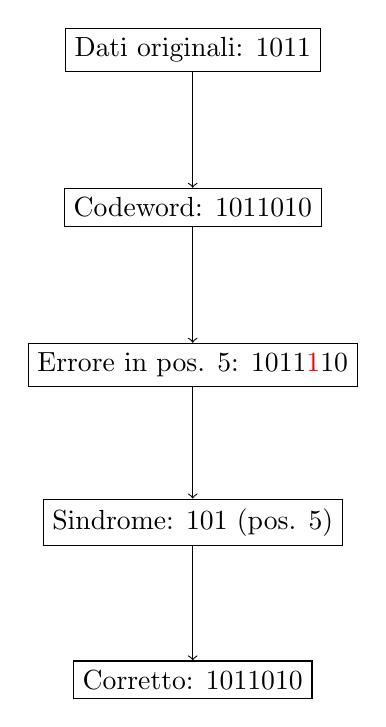
\begin{tikzpicture}[node distance=2cm]
\node[draw, rectangle] (orig) {Dati originali: 1011};
\node[draw, rectangle, below of=orig] (code) {Codeword: 1011010};
\node[draw, rectangle, below of=code] (error) {Errore in pos. 5: 1011\textcolor{red}{1}10};
\node[draw, rectangle, below of=error] (syndrome) {Sindrome: 101 (pos. 5)};
\node[draw, rectangle, below of=syndrome] (corrected) {Corretto: 1011010};

\draw[->] (orig) -- (code);
\draw[->] (code) -- (error);
\draw[->] (error) -- (syndrome);
\draw[->] (syndrome) -- (corrected);
\end{tikzpicture}
\end{center}

\subsubsection{4. Formula per il Numero di Bit di Parità}

\begin{center}
\fbox{$2^p \geq k + p + 1$}

\vspace{0.5cm}
\begin{tabular}{|c|c|c|}
\hline
Bit di dati (k) & Bit di parità (p) & Lunghezza totale (n) \\
\hline
4 & 3 & 7 \\
8 & 4 & 12 \\
11 & 4 & 15 \\
26 & 5 & 31 \\
\hline
\end{tabular}
\end{center}


\subsection{Consigli e Errori Comuni:}
\begin{itemize}
    \item \textbf{Bit vs Byte:} Estrema attenzione alle unità. Capacità di rete spesso in bit/s, dimensione file in Byte.
    \item \textbf{Kilo, Mega:} 1 KB = 1024 Byte, 1 MB = 1024 KB (per storage). Per networking, 1 kbps = 1000 bps, 1 Mbps = 1000 kbps. Gli esami a volte usano 1KB=1000B; chiarisci o segui la convenzione dell'esempio se presente.
    \item \textbf{Slow Start vs Congestion Avoidance:} Comprendi la differenza e quando si passa da una all'altra.
\end{itemize}

\section{Routing (Algoritmo di Dijkstra)}

\subsection{Concetti Chiave:}
\begin{itemize}
    \item \textbf{Algoritmo di Dijkstra:} Trova il cammino minimo (minor costo) da un nodo sorgente a tutti gli altri nodi in un grafo pesato con pesi non negativi.
    \item \textbf{Tabella di Routing:} Mantenuta da ogni router, indica per ogni rete di destinazione, quale è il prossimo hop (next hop router) e/o l'interfaccia di uscita da usare.
    \item \textbf{Link State Routing (es. OSPF):}
    \begin{enumerate}
        \item Ogni router scopre i suoi vicini e il costo del link verso di loro.
        \item Ogni router assembla queste informazioni in un Link State Packet (LSP).
        \item Gli LSP vengono inviati (flooding) a tutti gli altri router nella rete.
        \item Ogni router costruisce una mappa completa della topologia della rete.
        \item Ogni router esegue Dijkstra sulla mappa per calcolare i cammini minimi verso tutte le destinazioni e costruisce la sua tabella di routing.
    \end{enumerate}
\end{itemize}

\subsection{Procedura di Svolgimento (Dijkstra):}
\begin{enumerate}
    \item \textbf{Inizializzazione:}
    \begin{itemize}
        \item Nodo Sorgente (S): Costo = 0.
        \item Tutti gli altri nodi: Costo = $\infty$.
        \item Insieme N' = \{S\} (nodi il cui cammino minimo è noto).
        \item Per ogni nodo $v$ non in N', $D(v)$ = costo del link $(S,v)$ se esiste, altrimenti $\infty$. $p(v)$ = S.
    \end{itemize}
    \item \textbf{Iterazione:}
    \begin{itemize}
        \item Trova il nodo $w$ non in N' con il $D(w)$ minimo.
        \item Aggiungi $w$ a N'.
        \item Per ogni vicino $v$ di $w$ che non è in N':
        \begin{itemize}
            \item Se $D(w) + \text{costo}(w,v) < D(v)$:
            \begin{itemize}
                \item $D(v) = D(w) + \text{costo}(w,v)$
                \item $p(v) = w$ (il predecessore di $v$ nel cammino minimo da S è $w$)
            \end{itemize}
        \end{itemize}
    \item Ripeti il passo 2 finché tutti i nodi sono in N'.
    \item \textbf{Costruzione Tabella di Routing per il nodo sorgente S:}
        \item Per ogni destinazione \texttt{Dest}:
        \begin{itemize}
            \item Il costo minimo è $D(\text{Dest})$.
            \item Per trovare il \textit{prossimo hop} da S verso \texttt{Dest}: traccia a ritroso i predecessori $p()$ da \texttt{Dest} fino a che il predecessore è S. Il nodo subito dopo S in questo cammino è il prossimo hop. Oppure, se $p(\text{Dest})$ è $y$ e $p(y)$ è $z$ ... e $p(q)$ è S, allora il primo passo da S è verso $q$.
        \end{itemize}
    \end{itemize}
\end{enumerate}


\subsection{Consigli e Errori Comuni:}
\begin{itemize}
    \item \textbf{Precisione:} Dijkstra è un algoritmo meccanico, ma un errore di calcolo in un passo si propaga.
    \item \textbf{Aggiornamento Predecessori:} Non dimenticare di aggiornare $p(v)$ quando trovi un cammino migliore per $D(v)$.
    \item \textbf{Next Hop vs Predecessore:} La tabella di routing usa il \textit{prossimo hop} dalla sorgente, non il predecessore diretto della destinazione.
\end{itemize}

\section{Codifica del Segnale Wireless}

\subsection{Concetti Chiave:}
\begin{itemize}
    \item \textbf{Modulazione Digitale:} Processo di variazione di una o più caratteristiche di un'onda portante (ampiezza, frequenza, fase) in base a un segnale digitale.
    \item \textbf{M-PSK (Multiple Phase Shift Keying):}
    \begin{itemize}
        \item Tecnica di modulazione di fase. Utilizza $M$ diverse fasi per rappresentare i simboli.
        \item Ogni simbolo rappresenta $k = \log_2 M$ bit. Ad esempio, 8-PSK ha $M=8$ simboli, quindi $k=\log_2 8 = 3$ bit per simbolo.
        \item L'ampiezza della portante rimane costante.
        \item Le $M$ fasi sono tipicamente equispaziate attorno al cerchio unitario, date da $\phi_i = \frac{2\pi i}{M}$ radianti o $\frac{360^\circ i}{M}$ gradi, per $i = 0, 1, \ldots, M-1$.
        \item \textbf{Separazione Angolare:} La differenza di fase tra simboli adiacenti è $\Delta\phi = \frac{360^\circ}{M}$.
        \item \textbf{Regione di Decisione:} Per ogni simbolo, la regione di decisione si estende $\pm \frac{\Delta\phi}{2} = \pm \frac{360^\circ}{2M}$ attorno alla sua fase nominale. Se il segnale ricevuto (con rumore) cade al di fuori di questa regione, si verifica un errore di simbolo.
    \end{itemize}
    \item \textbf{M-QAM (Multiple Quadrature Amplitude Modulation):} Modula sia l'ampiezza che la fase della portante per ottenere più simboli. Permette più bit per simbolo rispetto a PSK a parità di $M$ (o M più elevati a parità di complessità di fase).
    \item \textbf{Costellazione:} Rappresentazione grafica dei simboli di modulazione nello spazio I/Q (In-phase / Quadrature). Ogni punto rappresenta un simbolo, che codifica uno o più bit.
    \item \textbf{Simbolo:} Un particolare stato dell'onda portante (es. una specifica ampiezza e fase).
    \item \textbf{Symbol Rate (Baud Rate):} Numero di simboli trasmessi al secondo (misurato in Baud).
    \item \textbf{Bit Rate:} Numero di bit trasmessi al secondo ($\text{Bit Rate} = \text{Symbol Rate} \times k$, dove $k = \text{bit\_per\_simbolo}$).
    \item \textbf{Gray Coding:}
    \begin{itemize}
        \item Una tecnica di etichettatura dei punti della costellazione (simboli) con sequenze di bit.
        \item \textbf{Scopo:} Minimizzare il numero di errori di bit quando si verifica un errore di simbolo, specialmente verso un simbolo adiacente (il tipo di errore più probabile a causa del rumore).
        \item Con Gray coding, le sequenze di bit assegnate a simboli adiacenti nella costellazione differiscono per un solo bit (distanza di Hamming = 1).
        \item \textbf{Esempio (8-PSK, 3 bit):} Una possibile sequenza Gray disposta attorno al cerchio PSK: 000 $\leftrightarrow$ 001 $\leftrightarrow$ 011 $\leftrightarrow$ 010 $\leftrightarrow$ 110 $\leftrightarrow$ 111 $\leftrightarrow$ 101 $\leftrightarrow$ 100 (e 100 $\leftrightarrow$ 000).
    \end{itemize}
    \item \textbf{SER (Symbol Error Rate):} Probabilità che un simbolo ricevuto sia diverso dal simbolo trasmesso.
    \item \textbf{BER (Bit Error Rate):} Probabilità che un bit ricevuto sia errato.
    \begin{itemize}
        \item Con Gray coding, un errore al simbolo più probabile (quello adiacente) causa tipicamente un solo errore di bit. In questo caso, BER $\approx$ SER / $k$ (se ogni errore di simbolo fosse verso un simbolo che causa un solo bit error), o più conservativamente, BER $\approx$ SER se si assume che la maggior parte degli errori di simbolo porti a un singolo errore di bit, specialmente in canali con SNR elevato dove gli errori a simboli non adiacenti sono rari. Per M-PSK, quando un errore di simbolo porta a un simbolo adiacente, si ha un solo errore di bit.
    \end{itemize}
    \item \textbf{Fase:} Spostamento temporale dell'onda rispetto a un riferimento. (Anticipo = fase positiva o $<$360\textdegree; Ritardo = fase negativa o $>$0\textdegree).
    \item \textbf{Ampiezza:} "Altezza" dell'onda.
\end{itemize}

\subsection{Procedura di Svolgimento (Interpretazione Encoding K/H):}
\begin{enumerate}
    \item \textbf{Analizza la Leggenda/Encoding:} Studia attentamente la figura che definisce la codifica (es. Encoding K o H nell'esame del 18 Feb 2021). Ogni punto della costellazione corrisponde a una sequenza di bit (solitamente 3 bit se ci sono 8 punti).
    \item \textbf{Segnale di Riferimento:} Comprendi il segnale $A \cdot \sin(B \cdot t)$ (fase zero, ampiezza A).
    \item \textbf{Decodifica i Simboli Ricevuti:}
    \begin{itemize}
        \item Per ogni "symbol duration" nel segnale ricevuto:
        \begin{itemize}
            \item Confronta la forma d'onda ricevuta con il segnale di riferimento.
            \item Determina la \textbf{fase} relativa (0\textdegree, 90\textdegree{} anticipo, 90\textdegree{} ritardo, 180\textdegree).
            \item Determina l'\textbf{ampiezza} relativa (es. "ampiezza $<$" o "ampiezza $>$" rispetto al riferimento, o due livelli specifici).
            \item Usa fase e ampiezza per trovare il punto corrispondente nella costellazione della codifica scelta (K o H).
            \item Leggi i bit associati a quel punto.
        \end{itemize}
    \item \textbf{Assembla la Sequenza di Bit.}
    \item \textbf{Conversione Esadecimale/Parità (se richiesto):}
    \begin{itemize}
        \item Dividi la sequenza di bit in gruppi di 8 (byte).
        \item Verifica la parità (se c'è un bit di parità per ogni byte).
        \item Converti i byte corretti in esadecimale.
    \end{itemize}
    \end{itemize}
\end{enumerate}

\subsection{Esempio Svolto (basato su Esercizio 2, "18 febbraio 2021" e Esercizio 10 "21 Luglio 2023"):}
Prendiamo l'Encoding K dell'esame del 18 Feb 2021 e la sequenza esadecimale OEAF... dell'esame del 21 Luglio 2023.

\textbf{Esercizio 10, "21 Luglio 2023":}
\begin{itemize}
    \item \texttt{Encoding K} (dall'altro esame, ma il principio è lo stesso):
    \begin{description}[font=\texttt\bfseries]
        \item[000:] ampiezza $<$, fase 0\textdegree
        \item[001:] ampiezza $>$, fase 0\textdegree{} (segnale riferimento)
        \item[010:] ampiezza $>$, fase 90\textdegree{} ritardo
        \item[011:] ampiezza $>$, fase 90\textdegree{} anticipo
        \item[100:] ampiezza $<$, fase 90\textdegree{} ritardo
        \item[101:] ampiezza $<$, fase 180\textdegree
        \item[110:] ampiezza $>$, fase 180\textdegree
        \item[111:] ampiezza $<$, fase 90\textdegree{} anticipo
    \end{description}
    \item \textbf{a) Sequenza esadecimale OEAF... $\to$ binario (primi 18 bit) + padding 00:}
    \begin{itemize}
        \item O (esadecimale) = \texttt{0000} (binario)
        \item E (esadecimale) = \texttt{1110} (binario)
        \item A (esadecimale) = \texttt{1010} (binario)
        \item F (esadecimale) = \texttt{1111} (binario)
        \item Sequenza binaria: \texttt{0000 1110 1010 1111}. Sono 16 bit. Ne servono 18.
        \item Completare a 18 bit aggiungendo zero a destra: \texttt{0000 1110 1010 1111 00}.
        \item La soluzione dell'esame dice: \texttt{0000 (O) 1110 (E) 1010 (A) 1111 (F) + 00 (padding)}
        \texttt{000 011 101 010 111 100} (raggruppati a 3 bit per simbolo)
    \end{itemize}
    \item \textbf{c) Simboli trasmessi (binario):}
    \texttt{000}, \texttt{011}, \texttt{101}, \texttt{010}, \texttt{111}, \texttt{100}
    \item \textbf{b) Forme d'onda (basate sulla mia interpretazione dell'Encoding K sopra):}
    \begin{enumerate}
        \item \texttt{000}: $\sin(t)$ con ampiezza ridotta, fase 0\textdegree.
        \item \texttt{011}: $\sin(t)$ con ampiezza piena, fase 90\textdegree{} anticipo (inizia dal picco positivo).
        \item \texttt{101}: $\sin(t)$ con ampiezza ridotta, fase 180\textdegree{} (inizia da zero andando verso il negativo).
        \item \texttt{010}: $\sin(t)$ con ampiezza piena, fase 90\textdegree{} ritardo (inizia dal picco negativo).
        \item \texttt{111}: $\sin(t)$ con ampiezza ridotta, fase 90\textdegree{} anticipo.
        \item \texttt{100}: $\sin(t)$ con ampiezza ridotta, fase 90\textdegree{} ritardo.
    \end{enumerate}
    \textit{Disegna queste forme d'onda nei box forniti, rispettando la durata del simbolo.}
\end{itemize}

\subsection{Consigli e Errori Comuni:}
\begin{itemize}
    \item \textbf{Leggere la Leggenda:} La chiave è capire la mappatura bit $\to$ simbolo (fase/ampiezza).
    \item \textbf{Fase 0 vs 180:} $\sin(t)$ a fase 0\textdegree{} inizia da 0 e va positivo. $\sin(t)$ a fase 180\textdegree{} inizia da 0 e va negativo.
    \item \textbf{Fase 90 Anticipo/Ritardo:} Anticipo (es. +90\textdegree) significa che l'onda è "spostata a sinistra" rispetto al riferimento; inizia prima nel suo ciclo. Ritardo (es. -90\textdegree{} o +270\textdegree) è spostata a destra. $\sin(t+90\textdegree) = \cos(t)$ (inizia dal picco). $\sin(t-90\textdegree) = -\cos(t)$ (inizia dal minimo).
    \item \textbf{Ampiezza:} Assicurati di distinguere i livelli di ampiezza correttamente.
\end{itemize}

\hrule % Linea orizzontale come separatore

\subsection{EIRP (Effective Isotropic Radiated Power)}
L'EIRP è la potenza totale che dovrebbe essere irradiata da un'antenna isotropica (che irradia uniformemente in tutte le direzioni) per produrre la stessa intensità di segnale (densità di potenza) nella direzione di massimo guadagno di un'antenna direzionale.

\begin{align*}
    \text{EIRP}_{\text{lin}} &= P_{\text{tx}} \cdot G_{\text{ant}} \cdot L_{\text{cavo}} \\
    \text{EIRP}_{\text{dB}} &= P_{\text{tx}}[\text{dBm}] + G_{\text{ant}}[\text{dBi}] - L_{\text{cavo}}[\text{dB}]
\end{align*}

\textbf{Esempio:} Se abbiamo:
\begin{itemize}
    \item Potenza trasmettitore: $P_{\text{tx}} = 100\text{ mW} = 20\text{ dBm}$ 
    \item Guadagno antenna: $G_{\text{ant}} = 15\text{ dBi}$
    \item Perdite cavo: $L_{\text{cavo}} = 2\text{ dB}$
\end{itemize}

Allora:
\[ \text{EIRP}_{\text{dB}} = 20\text{ dBm} + 15\text{ dBi} - 2\text{ dB} = 33\text{ dBm} \]

In milliwatt:
\[ \text{EIRP}_{\text{mW}} = 10^{33/10} \approx 1995\text{ mW} \approx 2\text{ W} \]

\subsection{Esempio Svolto (Calcolo EIRP e Potenza IR - Esercizio 12 Ripasso Finale)}
\begin{itemize}
    \item \textbf{Domanda 1:} Qual è il valore EIRP di un intentional radiator (IR) che fornisce 2W di segnale a un'antenna direzionale con guadagno di 18 dBi?
    \item \textbf{Soluzione 1:}
    \begin{enumerate}
        \item \textbf{Potenza dell'Intentional Radiator ($\text{P}_{\text{IR}}$) in dBm:}
        $\text{P}_{\text{IR}} = 2\text{W} = 2000\text{mW}$.
        Usando la conversione $P(\text{dBm}) = 10 \log_{10}(P(\text{mW}))$:
        \[ \text{P}_{\text{IR}}(\text{dBm}) = 10 \log_{10}(2000) = 10 \times (\log_{10}(2) + \log_{10}(1000)) \]
        \[ = 10 \times (0.301 + 3) = 10 \times 3.301 \approx 33.01 \text{ dBm} \]
        Oppure, con il metodo approssimato: $1\text{mW} = 0\text{dBm}$. $2000\text{mW} = 1\text{mW} \times 2 \times 10 \times 10 \times 10$.
        In scala dB: $0\text{dBm} + 3\text{dB} + 10\text{dB} + 10\text{dB} + 10\text{dB} = 33\text{dBm}$.
        \item \textbf{Guadagno antenna ($\text{G}_{\text{antenna}}$):}
        \[ \text{G}_{\text{antenna}} = 18 \text{ dBi} \]
        \item \textbf{Calcolo EIRP:}
        Assumendo perdite nei cavi trascurabili.
        \[ \text{EIRP(dBm)} = \text{P}_{\text{IR}}(\text{dBm}) + \text{G}_{\text{antenna}}(\text{dBi}) \]
        \[ \text{EIRP} = 33 \text{ dBm} + 18 \text{ dBi} = 51 \text{ dBm} \]
        \item \textbf{EIRP in Watt (per riferimento):}
        \[ \text{EIRP(mW)} = 10^{(\text{EIRP(dBm)}/10)} = 10^{(51/10)} = 10^{5.1} \text{ mW} \]
        \[ = 125892.5 \text{ mW} \approx 125.9 \text{ W} \]
        (L'approssimazione $2^{17} \text{mW} \approx 131 \text{W}$ è basata su diverse approssimazioni di dB). Il valore calcolato con la formula diretta è $125.9 \text{W}$.
    \end{enumerate}

    \item \textbf{Domanda 2:} E se il limite EIRP fosse di 40 mW, a quanto dovrebbe limitarsi il segnale IR (potenza fornita all'antenna) in tale sistema?
    \item \textbf{Soluzione 2:}
    \begin{enumerate}
        \item \textbf{Limite EIRP in dBm:}
        Limite EIRP $= 40\text{mW}$.
        \[ \text{Limite\_EIRP(dBm)} = 10 \log_{10}(40) = 10 \times (\log_{10}(4) + \log_{10}(10)) \]
        \[ = 10 \times (0.602 + 1) = 10 \times 1.602 \approx 16.02 \text{ dBm} \]
        Oppure, con il metodo approssimato: $40\text{mW} = 1\text{mW} \times 2 \times 2 \times 10$.
        In scala dB: $0\text{dBm} + 3\text{dB} + 3\text{dB} + 10\text{dB} = 16\text{dBm}$.
        \item \textbf{Calcolo potenza IR massima ($\text{P}_{\text{IR\_max}}$):}
        Sappiamo che $\text{EIRP(dBm)} = \text{P}_{\text{IR}}(\text{dBm}) + \text{G}_{\text{antenna}}(\text{dBi})$.
        Quindi, per rispettare il limite:
        \[ \text{P}_{\text{IR\_max}}(\text{dBm}) = \text{Limite\_EIRP(dBm)} - \text{G}_{\text{antenna}}(\text{dBi}) \]
        \[ \text{P}_{\text{IR\_max}} = 16 \text{ dBm} - 18 \text{ dBi} = -2 \text{ dBm} \]
        \item \textbf{Potenza IR massima in mW:}
        \[ \text{P}_{\text{IR\_max}}(\text{mW}) = 10^{(-2/10)} = 10^{-0.2} \text{ mW} \approx 0.631 \text{ mW} \]
        (L'approssimazione $1\text{mW} \times 10 / (2^4) = 0.625 \text{mW}$ data nell'esempio del prof è basata sul metodo approssimato: $-2\text{dBm} = (10 - 3 - 3 - 3 - 3)\text{dBm}$ rispetto a $0\text{dBm}$).
        Quindi, la potenza massima che l'IR può fornire all'antenna è circa $0.631 \text{mW}$ (o $0.625 \text{mW}$ con il metodo approssimato).
    \end{enumerate}
\end{itemize}

\end{document}